%&../.preamble
\endofdump

\usetikzlibrary{external}
\usepackage{cancel}
\usepackage{contour}
\tikzset{external/system call={pdflatex --shell-escape --fmt=../.preamble --halt-on-error -jobname "\image" "\endofdump\texsource"}}
\tikzexternalize[prefix=tikz/]

\newcommand{\inputGrammar}[1]{
	\input{|"node table_generator/grammar.js #1"}

	\begin{center}
		\input{|"node table_generator/first_follow.js #1"}
	\end{center}

	\begin{table}[H]
		\begin{center}
			\input{|"node table_generator/table.js #1"}
		\end{center}
		\caption{Tabella LR(0) \textit{senza} pruning}
	\end{table}

	\begin{table}[H]
		\begin{center}
			\input{|"node table_generator/table.js #1 --pruned"}
		\end{center}
		\caption{Tabella LR(0) \textit{con} pruning}
	\end{table}
}

\title{Linguaggi formali e compilatori}
\author{Marini Mattia}
\date{$ 1^o $ semestre $ 3^o $ anno}

\begin{document}
\maketitle
\tableofcontents
\listofdefs
\listoftheorems
\newpage

\section{Grammatiche libere}
\subsection{Proprietà grammatiche libere}
\begin{teorema}{Chiusura linguaggi liberi rispetto a unione}\label{chiusura per unione}
	I linguaggi liberi sono chiusi relativamente all'unione. In altre parole dato $ \mathcal{L}_1 $ e $ \mathcal{L}_2 $, allora
	\[
		\mathcal{L}_1 \cup \mathcal{L}_2
	\]
	è libero
\end{teorema}
Per dimostrare che ciò è vero, basta creare la seguente grammatica
\[
	\mathcal{G}=\left(V_1^{\prime} \cup V_2^{\prime} \cup\{S\}, T_1 \cup T_2, S, \mathcal{P}_1^{\prime} \cup \mathcal{P}_2^{\prime} \cup\left\{S \rightarrow S_1^{\prime} | S_2^{\prime}\right\}\right)
\]

\begin{teorema}{Chiusura linguaggi liberi rispetto a concatenazione}\label{chiusura per concatenazione}

	I linguaggi liberi sono chiusi relativamente alla concatenazione. In altre parole dato $ \mathcal{L}_1 $ e $ \mathcal{L}_2 $, allora
	\[
		\mathcal{L}_1 \mathcal{L}_2
	\]
	è libero
\end{teorema}
Per dimostrare che ciò è vero, basta creare la seguente grammatica
\[
	\mathcal{G}=\left(V_1^{\prime} \cup V_2^{\prime} \cup\{S\}, T_1 \cup T_2, S, \mathcal{P}_1^{\prime} \cup \mathcal{P}_2^{\prime} \cup\left\{S \rightarrow S_1^{\prime}  S_2^{\prime}\right\}\right)
\]

In ambi i casi è importante che non ci sia sovrapposizione dei non terminali. Per evitare ciò basta usare un \underline{refresh} dei simboli non terminali

\begin{teorema}{NON chiusura dei linguaggi liberi rispetto all'intersezione}
	I linguaggi liberi NON sono chiusi relativamente all'intersezione. In altre parole dato $ \mathcal{L}_1 $ e $ \mathcal{L}_2 $, allora
	\[
		\mathcal{L}_1 \cap \mathcal{L}_2
	\]
	NON è libero
\end{teorema}
Per dimostrare si può considerare
\begin{itemize}
	\item $ \mathcal{L_1} = \left\{a^{n}b^{n}\right\} $ libero
	\item $ \mathcal{L_2} = \left\{c^{n}\right\} $ libero
	\item $ \mathcal{L}_3 = \mathcal{L}_1 \mathcal{L}_2 = \left\{a^{n}b^{n} c^{j}\right\}$ libero per teorema \ref{chiusura per concatenazione}
	\item

\end{itemize}
Se ora considero:
\begin{itemize}
	\item  $ \mathcal{L}_1 = \left\{a^{n}b^{n} c^{j}\right\}$
	\item  $ \mathcal{L}_2 = \left\{a^{j}b^{n}c^{n}\right\}$
\end{itemize}
la cui intersezione è $ \left\{a^{n}b^{n}c^{n}\right\} $, NON è libero. Quest'ultimo fatto è dimostrabile con il \hyperref[pumping lemma]{pumping lemma}


\subsection{Chomsky normal form}\label{chomsky normal form}
\begin{definizione}{Forma normale di chomsky}
	Una grammatica è in forma normale di Chomsky se ogni produzione è di una delle seguenti forme:
	\begin{itemize}
		\item $ A \rightarrow BC $
		\item $ A \rightarrow b $
	\end{itemize}
	Dove $ A, B, C $ sono non terminali e $ b $ è terminale
\end{definizione}
\subsubsection{Riduzione in forma di chomsky}
E' sempre possibile ridurre una grammatica libera in forma di chomsky seguendo i seguenti passaggi:
\begin{itemize}
	\item \sfblue{Eliminazione delle $ \epsilon $- produzioni}
	      \begin{itemize}
		      \item Per ogni produzione $ A \rightarrow Y_1 Y_2 \ldots Y_N $ considero tutti gli $ Y_i $ annullabili
		      \item Aggiungo tutte le possibili combinazioni di body che includano o meno i non terminali annullabili
		      \item Elimino ogni produzione $ A \rightarrow \epsilon $
	      \end{itemize}
	      Ad esempio, con $ X_1, X_2, X_3 $ annullabili, la produzione $ A \rightarrow aX_1BX_2X_3cD $ va spezzata in:
	      \begin{center}
		      \begin{tabular}{c c c c c c c}
			      \toprule
			      $a$   & $X_1$   & $B$   & $X_2$   & $X_3$ & $c$ & $D$ \\
			      \midrule
			      $ a $ & $ X_1 $ & $ B $ & $ X_2 $ & $X_3$ & $c$ & $D$ \\
			      $ a $ & $ X_1 $ & $ B $ & $ X_2 $ &       & $c$ & $D$ \\
			      $ a $ & $ X_1 $ & $ B $ &         & $X_3$ & $c$ & $D$ \\
			      $ a $ & $ X_1 $ & $ B $ &         &       & $c$ & $D$ \\
			      $ a $ &         & $ B $ & $ X_2 $ & $X_3$ & $c$ & $D$ \\
			      $ a $ &         & $ B $ & $ X_2 $ &       & $c$ & $D$ \\
			      $ a $ &         & $ B $ &         & $X_3$ & $c$ & $D$ \\
			      $ a $ &         & $ B $ &         &       & $c$ & $D$ \\

			      % $ a $ &         & $ B $ &       & $X_3$ & $c$ & $D$ \\
			      % $ a $ &         & $ B $ &       &       & $c$ & $D$ \\
			      % $ a $ &         & $ B $ & $X_2$ & $X_3$ & $c$ & $D$ \\
			      % $ a $ &         & $ B $ & $X_2$ &       & $c$ & $D$ \\
			      % $ a $ & $ X_1 $ & $ B $ &       & $X_3$ & $c$ & $D$ \\
			      % $ a $ & $ X_1 $ & $ B $ &       &       & $c$ & $D$ \\
			      % $ a $ & $ X_1 $ & $ B $ & $X_2$ & $X_3$ & $c$ & $D$ \\
			      % $ a $ & $ X_1 $ & $ B $ & $X_2$ &       & $c$ & $D$ \\
			      \bottomrule
		      \end{tabular}
	      \end{center}
	      dando origine ai seguenti body:
	      \begin{align*}
		       & aX_1BX_2X_3cD                      &  & a    X_1    B    X_2          c  D   &  & a    X_1    B            X_3  c  D   &  & a    X_1    B                   c  D   \\
		       & a             B    X_2   X_3  c  D &  & a             B    X_2          c  D &  & a             B            X_3  c  D &  & a             B                   c  D
	      \end{align*}

	\item \sfblue{Eliminazione dei non terminali inutili} (ossia dei non terminali che \textit{non} compaiono in nessuna produzione)
	\item \sfblue{Eliminazione delle unity productions}
	      \begin{itemize}
		      \item Dato $ B \rightarrow \alpha \mid \beta  $, sostituisco ogni produzione $ A \rightarrow B $ con
		            \[
			            A \rightarrow \alpha \mid \beta
		            \]
	      \end{itemize}
	\item \sfblue{Spezzettamento body troppo lunghi}
	      \begin{itemize}
		      \item Ad esempio prendo $ S \rightarrow a S b \mid a b $
		      \item Ogni terminale lo sostituisco con una nuova produzione:
		            \[
			            S \rightarrow ASB \mid AB \quad A \rightarrow b \quad B \rightarrow b
		            \]
		      \item Ogni stringa di non terminali con lunghezza $ \ge 3 $ la spezzo inserendo un nuovo non terminale:
		            \[
			            S \rightarrow AC \mid AB \quad C \rightarrow SB \quad A \rightarrow b \quad B \rightarrow b
		            \]
	      \end{itemize}
\end{itemize}
\subsection{Pumping lemma}\label{pumping lemma}
\begin{teorema}{Pumping lemma}
	Dato un linguaggio libero $ \mathcal{L}\left(\mathcal{G}\right) $, allora:
	\begin{itemize}
		\item Dato $ p \ge 0 $
		\item $ \forall z \text{ t.c. } \left|z\right| > p $ valgono le seguenti condizioni:
		\item Allora esiste un \textit{"unpacking"} di $ z $, ossia $ z = uvwxy $ tali per cui
		      \begin{itemize}
			      \item $ \left|vwx\right| \le p $
			      \item $ \left|uv\right| > 0$
			      \item $ \forall i \in \N \quad u v^{i}w x^{i}y \in \mathcal{L}\left(\mathcal{G}\right) $
		      \end{itemize}
	\end{itemize}
\end{teorema}
Informalmente, posso "pompare" all'infinito la lunghezza di parole abbastanza lunghe se il linguaggio è libero o, al contrario, le parole abbastanza lunghe possono essere ottenute solo tramite "pumping"

\subsubsection{Dimostrazione}
Considero la grammatica in forma normale di Chomski. Questo è sempre possibile come descritto in sezione \ref{chomsky normal form}. Questo è utile in quanto un albero di derivazione di una una parola in una grammatica in Chomsky normal form è un \textit{albero binario}
\begin{itemize}
	\item Considero una parola $ z $ con $ \left|z\right| \ge 2^{k+1} $ dove $ k $ è il numero di non terminali distinti della grammatica
	      \[
		      p = 2^{k+1}
	      \]
	\item L'albero di derivazione di $ z $ ha altezza $ \ge k+1 $, dato che il caso in cui l'altezza è minima a parità di numero di foglie è quello in cui l'albero è completo
	\item Un path dalla root alla foglia di lunghezza massima ha $ k + 2 $ nodi, di cui $ k+1 $ sono \textit{non terminali}, dunque ho la certezza che \textit{esista} almeno un non terminale ripetuto
	\item Fra i non terminali ripetuti, chiamo $ A $ quello la cui seconda occorrenza a partire dal basso sia più bassa
	\item Ora considero il seguente unpacking:
	      \begin{center}
		      \begin{tikzpicture}[scale = 1.4]
			      \draw [dashed](-3,0)--(3,0)--(0,5)--cycle;
			      \draw [thick](-2,0)--(2,0)--(0,3)--cycle;
			      \draw (-1,0)--(1,0)--(0,1)--cycle;
			      \node [anchor=north] at (-2.5, 0) {$u$};
			      \node [anchor=north] at (-1.5, 0) {$v$};
			      \node [anchor=north] at (0, 0)    {$w$};
			      \node [anchor=north] at (1.5, 0)  {$x$};
			      \node [anchor=north] at (2.5, 0)  {$y$};
			      \node (a1)[anchor = south] at (0, 1) {$ A_1 $};
			      \node (a2)[anchor = south] at (0, 3) {$ A_2 $};
			      \node (s)[anchor = south] at (0, 5) {$ S $};
			      \draw [dotted](a1)decorate [decoration={zigzag,segment length=16pt}]{ -- (a2)};
			      \draw [dotted](s)decorate [decoration={zigzag,segment length=16pt}]{ -- (a2)};
		      \end{tikzpicture}
	      \end{center}
	      \begin{itemize}
		      \item $ \left|uwx\right| \le p $ in quanto:
		            \begin{itemize}
			            \item Ho selezionato $ A_2 $ in maniera tale che fosse il primo carattere ripetuto partendo dal basso.
			            \item Per questo il sottoalbero radicato in $ A_2 $ ha al più altezza $ k $, quindi al più avrà $ 2^{k} $ foglie
		            \end{itemize}
		      \item $ \left|vx\right| > 0 $ in quanto non esistono produzioni unitarie nella forma normale di Chomsky
	      \end{itemize}
\end{itemize}

\section{Top down parsing}
Prendiamo ora come esempio una grammatica libera:
\begin{align*}
	E  & \rightarrow  TE'                \\
	E' & \rightarrow  +TE' \mid \epsilon \\
	T  & \rightarrow  FT'                \\
	T' & \rightarrow  *FT' \mid \epsilon \\
	F  & \rightarrow  (E) \mid \text{id}
\end{align*}\label{grammatica esempio}

\begin{definizione}{First($ \alpha  $)}
	Data una grammatica e una qualsiasi stringa $ \alpha  $, $ \operatorname{first}\left(\alpha \right) $ sono i caratteri terminali che possono comparire all'inizio della stringa dopo una sua qualsiasi espansione
\end{definizione}
Operativamente, per trovare i first:
\begin{itemize}
	\item Prendo una derivazione $ A \rightarrow XYZ $
	\item Se $ X $ è terminale allora lo aggiungo a first($ \alpha  $)
	\item Se $ X $ è non terminale allora aggiundo $ \operatorname{first}\left(X\right) $ a $ \operatorname{first}\left(\alpha \right) $
	\item Se $ X $ è \textit{annullabile}, allora devo controllare anche i first($ Y $) (se $ X \rightarrow * \varepsilon  $ allora la stringa inizia per $ Y $)
\end{itemize}
\begin{definizione}{Follow(A)}
	Data una grammatica e un qualsiasi non terminale $ A $, $ \operatorname{follow}\left(A\right) $ sono i caratteri che possono seguire $ A $ dopo una qualsiasi espansione
\end{definizione}
Operativamente, per trovare i follow(A):
\begin{itemize}
	\item Prendo ogni derivazione $ B \rightarrow \alpha A \beta $
	\item Aggiungo i $ \operatorname{first}\left(\beta \right) $ a $ \operatorname{follow}\left(A\right) $
	\item Se $ \beta  $ è \textit{annullabile}, allora aggiungo $ \operatorname{follow}\left(B\right) $ a $ \operatorname{follow}\left(A\right) $
\end{itemize}
Quest'ultima condizione è data dal fatto che
\begin{center}
	\begin{forest}
		for tree={grow = -90}
		[ ...
			[$ B $
				[$ \alpha  $]
					[$ A $, name=a]
					[\textcolor{gray!50}{$ \beta $}, tier=2]
			]
			[follow(B), name = follow, edge={dotted}, tier = 2]
		]
		\draw [bend right](a.south) to(follow.south);
	\end{forest}
\end{center}


\subsubsection{Esempio 1 first follow}
Sempre in riferimento a \hyperref[grammatica esempio]{questa grammatica}, vediamo come calcolare i first e follow:

\begin{minipage}[t]{0.48\textwidth}
	\begin{align*}
		E  & \rightarrow  TE'                \\
		E' & \rightarrow  +TE' \mid \epsilon \\
		T  & \rightarrow  FT'                \\
		T' & \rightarrow  *FT' \mid \epsilon \\
		F  & \rightarrow  (E) \mid \text{id}
	\end{align*}
\end{minipage}
%
\begin{minipage}[t]{0.48\textwidth}
	\begin{table}[H]
		\centering
		\begin{tabular}{l|ll}
			\toprule
			       & first()        & follow()      \\
			\midrule
			$ E $  & $\text{id}, ($ & $\$, )$       \\
			$ E' $ & $\epsilon, +$  & $\$, )$       \\
			$T $   & $\text{id}, ($ & $\$, ), +$    \\
			$T'$   & $\epsilon, *$  & $\$, ), +$    \\
			$F $   & $\text{id}, ($ & $\$, ), +, *$ \\
			\bottomrule
		\end{tabular}
	\end{table}
\end{minipage}

\subsubsection{Esempio 2 first follow}
\begin{minipage}[t]{0.48\textwidth}
	\begin{align*}
		S & \rightarrow  aABb            \\
		A & \rightarrow  Ac \mid d       \\
		B & \rightarrow  CD              \\
		C & \rightarrow  e \mid \epsilon \\
		D & \rightarrow  f \mid \epsilon
	\end{align*}
\end{minipage}
%
\begin{minipage}[t]{0.48\textwidth}
	\begin{table}[H]
		\centering
		\begin{tabular}{l|ll}
			\toprule
			      & first()          & follow()     \\
			\midrule
			$ S $ & $a$              & $\$$         \\
			$ A $ & $d$              & $b, c, e, f$ \\
			$ B $ & $e, f, \epsilon$ & $b$          \\
			$ C $ & $e, \epsilon$    & $b, f$       \\
			$ D $ & $f, \epsilon$    & $b$          \\
			\bottomrule
		\end{tabular}
	\end{table}
\end{minipage}

Nota che nel calcolo di follow(A), quando considero $ S \rightarrow aABb $, so che
\[
	\operatorname{follow\left(A\right)} = \operatorname{first\left(Bb\right)} + \operatorname{follow}\left(S\right)
\]
quindi non devo limiratmi ad aggiungere solo first($ B $)=$ e,f,\epsilon  $, bensì first($ Ab $) = $ e,f,\epsilon, b$

\subsubsection*{Esempio 3 first follow}
\begin{minipage}[t]{0.48\textwidth}
	\begin{align*}
		S & \rightarrow  aA \mid bBc     \\
		A & \rightarrow  Bd \mid Cc      \\
		B & \rightarrow  e \mid \epsilon \\
		C & \rightarrow  f \mid \epsilon
	\end{align*}
\end{minipage}
%
\begin{minipage}[t]{0.48\textwidth}
	\begin{table}[H]
		\centering
		\begin{tabular}{l|ll}
			\toprule
			      & first()       & follow() \\
			\midrule
			$ S $ & $a, b$        & $\$$     \\
			$ A $ & $e, d, f, c$  & $\$$     \\
			$ B $ & $e, \epsilon$ & $c, d$   \\
			$ C $ & $f, \epsilon$ & $c$      \\
			\bottomrule
		\end{tabular}
	\end{table}
\end{minipage}

\subsection{Costruzione tabella di parsing}\label{parsing table}
La tabella di parsing può essere costruita secondo la seguente intuizione:
\begin{center}
	Prendo ogni non terminale e lo assegno ad ogni riga, prendo ogni terminale e lo assegno ad ogni colonna. \verb|m[i][j]| è riempita se e solo se esiste qualche produzione che trasformi il non terminale $ i $ in una stringa che incomincia per $ j $.
\end{center}
Operativamente per ogni produzione $ A \rightarrow \alpha  $:
\begin{itemize}
	\item \sfblue{Aggiungo} tutti i first($ \alpha $)
	\item Se $ \alpha  $ è annullabile ($ \epsilon \in \operatorname{first}\left(\alpha \right)  $) allora \sfblue{aggiungo} tutti i follow(A)
\end{itemize}
Con \sfblue{aggiungo} indico il fatto che la cella $ m\left[A\right]\left[c\right] $ viene riempita con la produzione $ A \rightarrow \alpha $
\vskip3mm
In altri termini
\begin{itemize}
	\item Per ogni riga della tabella avrò una o più produzioni
	\item Per ogni produzione controllo quali caratteri $ C $ posso ottenere all'inizio di una qualsiasi stringa
	\item Aggiungo questa produzione nelle celle della riga corrente in corrispondenza di ogni carattere $ c $ trovato
\end{itemize}
Ad esempio, una tabella di parsing per la \hyperref[grammatica esempio]{grammatica d'esempio}

\begin{table}[H]
	\centering
	\begin{tabular}{c|c|c|c|c|c|c}
		\toprule
		     & $id$                & $+$                       & $*$                   & $($                 & $)$                       & $\$$                      \\
		\midrule
		$E$  & $E \rightarrow TE'$ &                           &                       & $E \rightarrow TE'$ &                           &                           \\
		\hline
		$E'$ &                     & $E' \rightarrow +TE'$     &                       &                     & $E' \rightarrow \epsilon$ & $E' \rightarrow \epsilon$ \\
		\hline
		$T$  & $T \rightarrow FT'$ &                           &                       & $T \rightarrow FT'$ &                           &                           \\
		\hline
		$T'$ &                     & $T' \rightarrow \epsilon$ & $T' \rightarrow *FT'$ &                     & $T' \rightarrow \epsilon$ & $T' \rightarrow \epsilon$ \\
		\hline
		$F$  & $F \rightarrow id$  &                           &                       & $F \rightarrow (E)$ &                           &                           \\
		\bottomrule
	\end{tabular}
	\caption{Tabella di parsing LL(1) per il \hyperref[grammatica esempio]{questa grammatica}}
\end{table}
\vskip3mm
\begin{minipage}[t]{0.48\textwidth}
	\begin{align*}
		E  & \rightarrow  TE'                \\
		E' & \rightarrow  +TE' \mid \epsilon \\
		T  & \rightarrow  FT'                \\
		T' & \rightarrow  *FT' \mid \epsilon \\
		F  & \rightarrow  (E) \mid \text{id}
	\end{align*}
\end{minipage}
%
\begin{minipage}[t]{0.48\textwidth}
	\begin{table}[H]
		\centering
		\begin{tabular}{l|ll}
			\toprule
			       & first()        & follow()      \\
			\midrule
			$ E $  & $\text{id}, ($ & $\$, )$       \\
			$ E' $ & $\epsilon, +$  & $\$, )$       \\
			$T $   & $\text{id}, ($ & $\$, ), +$    \\
			$T'$   & $\epsilon, *$  & $\$, ), +$    \\
			$F $   & $\text{id}, ($ & $\$, ), +, *$ \\
			\bottomrule
		\end{tabular}
	\end{table}
\end{minipage}
\vskip3mm
Nota che se il linguaggio è \underline{LL(1)} allora non avrò celle con due produzioni
\subsection{Parsing}\label{parsing}
Una volta costruita la tabella di parsing \hyperref[parsing table]{come descritto qui}, posso verificare se una stringa appartiene ad una grammatica eseguiendone il parsing. L'algoritmo di appoggia su uno \textit{stack} e procedere come segue:
\begin{itemize}
	\item Lo stack contiene l'espansione parziale della parola. Inizialmente contiene solo $ S $, ossia \textit{lo starting symbol}
	\item Tengo un puntatore al carattere della parola che sto cercando di ottenere. Inizialmente questo è settato al primo carattere
	\item Scorro e considero \verb|top| e \verb|c|, rispettivamente il primo carattere dello stack e il carattere correntemente puntato:
	      \begin{itemize}
		      \item Se \verb|top| è terminale e \verb|c == top| allora significa che sono riuscito ad espandere qualcosa e ottenere il carattere desiderato. Dunque avanzo il puntatore al carattere successivo
		      \item Se \verb|c != top| devo trovare un modo per espandere \verb|top| in \verb|c|. Controllo la tabella di parsing in \verb|m[top][c]|. Se ho una produzione la seguo, ossia rimuovo \verb|top| dallo stack e inserisco il body della produzione
		      \item In tutti gli altri casi non posso procedere perchè la parola non appartiene al linguaggio. In particolare può succedere che:
		            \begin{itemize}
			            \item \verb|top| è terminale ma diverso da \verb|b|
			            \item \verb|top| è non terminale ma non ho una produzione in \verb|m[top][c]| significa che la parola non appartiene al linguaggio
		            \end{itemize}
	      \end{itemize}
\end{itemize}
\subsection{Left recursion}
\begin{definizione}{Left recursive grammar}
	Una grammatica è left recursive se per qualche $ A $ ho che $ A \rightarrow^* A \alpha  $
\end{definizione}
Ad esempio, la grammatica
\begin{align*}
	S & \rightarrow B \mid a  \\
	B & \rightarrow Sa \mid b
\end{align*}
è \textit{left recursive}. Se espando $ S \rightarrow B \rightarrow Sa \rightarrow Ba \rightarrow Saa  \ldots  $ e così via


\begin{definizione}{Immediately left recursive grammar}
	Una grammatica è imeddiatamente left recursive se per qualche $ A $ ho che $ A \rightarrow A \alpha  $
\end{definizione}
Ad esempio,la grammatica:
\begin{align*}
	S \rightarrow Sa | b
\end{align*}
è \textit{immediately left recursive}. Infatti, espandendo $ S \rightarrow Sa \rightarrow Saa  \ldots  $ e così via

\begin{teorema}{Left recursion e LL(1) parsing}
	Se una grammatica è left recursive allora non può essere parsata con un parser LL(1)
\end{teorema}
Intuitivamente, supponendo di avere $ S \rightarrow S \alpha | a $, in un parser come descritto in sezione \ref{parsing} e una stringa $ a \alpha \alpha $
\vskip3mm
\begin{minipage}[t]{0.48\textwidth}
	\begin{center}
		\begin{tabular}{l|ll}
			\toprule
			      & first & follow          \\
			\midrule
			$ S $ & $ a $ & $ \$, \alpha  $ \\
			\bottomrule
		\end{tabular}
	\end{center}
\end{minipage}
%
\begin{minipage}[t]{0.48\textwidth}
	\begin{center}
		\begin{tabular}{l|l|l|l}
			\toprule
			  & $ \alpha $ & a                                                             & \$ \\
			\midrule
			S &            & $ S \rightarrow a $  \textbf{and} $ S \rightarrow S \alpha  $ &    \\
			\bottomrule
		\end{tabular}
	\end{center}
\end{minipage}
\vskip3mm
L'idea è che se ho una ricorsione a sinistra del tipo $ A \rightarrow A \alpha \mid \beta   $, allora avrò sempre due produzioni che mi permettono di arrivare a $ \beta $:
\begin{itemize}
	\item $ A \rightarrow A \alpha  \rightarrow  \beta \alpha  $
	\item $ A \rightarrow \beta $
\end{itemize}
quindi avrò sempre un conflitto nella tabella di parsing


\subsubsection{Grafo dei riferimenti}\label{grafo dei riferimenti}
Sta roba la ho inventata a cazzo di cane ma aiuta con la ricorsione.
\begin{definizione}{Grafo dei riferimenti}
	Data una grammatica $ G $, un grafo dei riferimenti è un grafo che ha come nodi i driver delle produzioni.
	Fra il nodo $ A $  e $ B $ esiste un arco se e solo se nel corpo di almeno una produzione con driver $ A $ compare $ B $
\end{definizione}
Se esiste un ciclo in questo grafo c'è qualche tipo di ricorsione. Nel ciclio ogni arco $ \left(A,B\right) $ corrisponde a una produzione di tipo $ A \rightarrow B \alpha $, allora la grammatica è \textit{left recursive}. Per esempio
\vskip3mm
\begin{minipage}[c]{0.48\textwidth}
	\begin{align*}
		A & \rightarrow Ba \mid b          \\
		B & \rightarrow  Bc \mid Ad \mid b
	\end{align*}
\end{minipage}
%
\begin{minipage}[c]{0.48\textwidth}
	\centering
	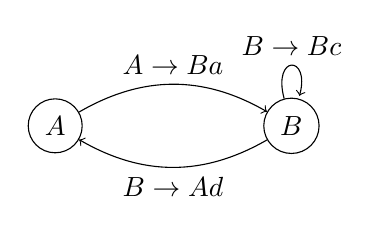
\begin{tikzpicture}
		\node (a)[circle, draw] at (0,0) {$ A $};
		\node (b)[circle, draw] at (3,0) {$ B $};
		\draw [bend left, ->](a)edge node [midway, above]{$ A \rightarrow Ba $}(b);
		\draw [bend left, ->](b)edge node [midway, below]{$ B \rightarrow Ad $}(a);
		\draw [-latex](b)edge[loop above] node [midway, above]{$ B \rightarrow Bc $} (b);
	\end{tikzpicture}
\end{minipage}
\subsubsection{Eliminazione immediate left recursion}\label{eliminazione left recursion}
La ricorsione sinistra immediata può essere eliminata in modo abbastanza semplice. Supponiamo di avere:
\[
	S \rightarrow S \alpha  \mid \beta
\]
che è un linguaggio che genera stringhe di tipo $ \beta \alpha^{n}  $. Posso introdurre un fresh non terminal per eseguire una ricorsione a destra anzichè a sinistra:
\begin{align*}
	S  & \rightarrow \beta  \mid \beta S'    \\
	S' & \rightarrow \alpha S' \mid \epsilon
\end{align*}
Ad esempio, prendendo $ \beta \alpha \alpha \alpha  $
\vskip3mm
\begin{minipage}[t]{0.48\textwidth}
	\begin{center}
		\begin{forest}
			for tree={grow = -90}
			[S
				[S
						[S
								[S
										[$ \beta $]
								]
								[$ \alpha $]
						]
						[$ \alpha $]
				]
				[$ \alpha $]
			]
		\end{forest}
		\vskip3mm
		Grammatica 1
	\end{center}
\end{minipage}
%
\begin{minipage}[t]{0.48\textwidth}
	\begin{center}
		\begin{forest}
			for tree={grow = -90}
			[S
				[$ \beta $]
				[$ S' $
					[$ \alpha  $]
						[$ S' $
							[$ \alpha  $]
								[$ S' $
									[$ \alpha  $]
										[$ S' $]
								]
						]
				]
			]
		\end{forest}
		\vskip3mm
		Grammatica 2
	\end{center}
\end{minipage}
\vskip3mm
Più in generale possiamo procedere così:
\begin{teorema}{Eliminazione ricorsione sinistra immediata}
	Se abbiamo una grammatica \textit{left recursive}, possiamo eliminare la ricorsione sinistra ottenendo una grammatica equivalente. In particolare, possiamo sostituire delle produzioni di questa forma
	\begin{align*}
		A \rightarrow A\alpha_1 \mid \ldots \mid A\alpha_n \mid \beta_1 \mid \ldots \mid \beta_k
	\end{align*}

	Dove $\alpha_j \neq \epsilon$ per ogni $j = 1 \ldots n$ e $\beta_i \neq A\gamma_i$ per ogni $i = 1 \ldots k$
	\vskip3mm
	con produzioni di quest'altra:

	\begin{align*}
		A  & \rightarrow \beta_1A' \mid \ldots \mid \beta_kA'                 \\
		A' & \rightarrow \alpha_1A' \mid \ldots \mid \alpha_nA' \mid \epsilon
	\end{align*}
\end{teorema}
L'idea è sempre la stessa. La grammatica genera una stringa nella forma:
\[
	\left\{w_1w_2 \mid w_1 \in \left\{\beta_1, \ldots, \beta_k\right\}, w_2 \in \left\{\alpha_1, \ldots, \alpha_n\right\}^{*} \right\}
\]
quindi posso
\begin{itemize}
	\item Dare la possibilità di espandere $ A $ in tutti i possibili $ \beta  $ ($ A $)
	\item Pushare dopo il $ \beta  $ scelto un numero arbitrario di $ \alpha $ ($ A' $)
\end{itemize}
\subsubsection{Eliminazione left recursion}
Per eliminare in generale la \textit{left recursion} posso
\begin{itemize}
	\item Riporto la grammatica ad una situazione in cui esiste solo \textit{immediate} left recursion
	\item Elimino la \textit{immediate left recursion come descritto} in sezione \ref{eliminazione left recursion}
\end{itemize}
Per effettuare il primo punto posso utilizzare il \hyperref[grafo dei riferimenti]{grafo dei riferimenti} (sez \ref{grafo dei riferimenti}). Se esiste un ciclo devo eliminarlo modificando un arco $ \left(A,B\right) $ a $ \left(A, A\right) $
Prendiamo per esempio:
\vskip3mm
\begin{minipage}[c]{0.48\textwidth}
	\begin{align*}
		A & \rightarrow Ba \mid b          \\
		B & \rightarrow  Bc \mid Ad \mid b
	\end{align*}
\end{minipage}
%
\begin{minipage}[c]{0.48\textwidth}
	\centering
	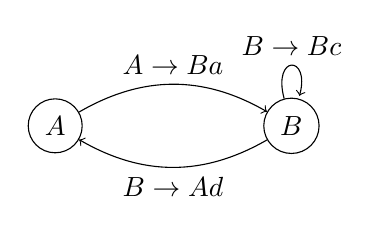
\begin{tikzpicture}
		\node (a)[circle, draw] at (0,0) {$ A $};
		\node (b)[circle, draw] at (3,0) {$ B $};
		\draw [bend left, ->](a)edge node [midway, above]{$ A \rightarrow Ba $}(b);
		\draw [bend left, ->](b)edge node [midway, below]{$ B \rightarrow Ad $}(a);
		\draw [-latex](b)edge[loop above] node [midway, above]{$ B \rightarrow Bc $} (b);
	\end{tikzpicture}
\end{minipage}
\vskip3mm
Posso prendere l'arco $ \left(B,A\right) $ e farlo puntare a $ B $ stesso
\begin{center}
	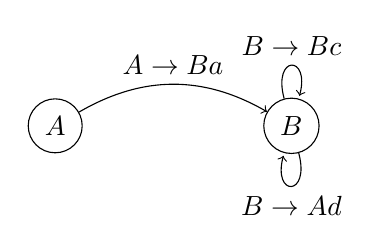
\begin{tikzpicture}
		\node (a)[circle, draw] at (0,0) {$ A $};
		\node (b)[circle, draw] at (3,0) {$ B $};
		\draw [bend left, ->](a)edge node [midway, above]{$ A \rightarrow Ba $}(b);

		\draw (b)edge[loop below]node [midway, below]{$ B \rightarrow Ad $} (b);
		\draw [-latex](b)edge[loop above] node [midway, above]{$ B \rightarrow Bc $} (b);
	\end{tikzpicture}
\end{center}
Per "reindirizzare" la produzione $ B \rightarrow Ad $, ed eliminare il riferimento di $ A $ da parte di $ B $, "includo" direttamente tutte le produzioni di $ A $ nella produzione che sto "reindirizzando":
\[
	B \rightarrow Ad
\]
diventa
\[
	B \rightarrow Bad \mid bd
\]
Di fatto, graficamente, nel nel grafo delle dipendenze prendo un arco $ \left(A, B\right) $ che voglio reindizizzare e
\begin{itemize}
	\item Ottengo un nuovo grafo in cui ho eliminato $ \left(A, B\right) $
	\item Ho un nuovo arco uscente da $ A $ che punta nella posizione di ogni arco uscente da $ B $
\end{itemize}
Nota che se esiste un self loop nel nodo di arrivo, allora non posso "reindirizzare" la produzione. Ad esempio
\begin{center}
	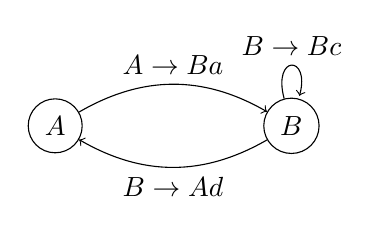
\begin{tikzpicture}
		\node (a)[circle, draw] at (0,0) {$ A $};
		\node (b)[circle, draw] at (3,0) {$ B $};
		\draw [bend left, ->](a)edge node [midway, above]{$ A \rightarrow Ba $}(b);
		\draw [bend left, ->](b)edge node [midway, below]{$ B \rightarrow Ad $}(a);
		\draw [-latex](b)edge[loop above] node [midway, above]{$ B \rightarrow Bc $} (b);
	\end{tikzpicture}
\end{center}
se reindirizzassi $ \left(A, B\right) $ non riuscirei ad eliminare il riferimento a $ B $ in $ A $, in quanto otterrei:

\begin{center}
	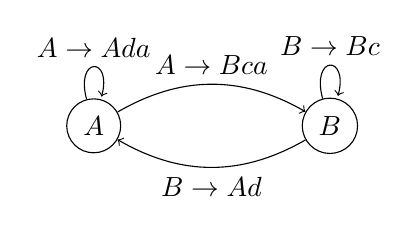
\begin{tikzpicture}
		\node (a)[circle, draw] at (0,0) {$ A $};
		\node (b)[circle, draw] at (3,0) {$ B $};
		\draw [bend left, ->](a)edge node [midway, above]{$ A \rightarrow Bca $}(b);
		\draw [bend left, ->](b)edge node [midway, below]{$ B \rightarrow Ad $}(a);

		\draw [-latex](b)edge[loop above] node [midway, above]{$ B \rightarrow Bc $} (b);
		\draw [-latex](a)edge[loop above] node [midway, above]{$ A \rightarrow Ada $} (a);
	\end{tikzpicture}
\end{center}

Quindi nel caso vi fosse un \textit{self loop} sinistro su qualsiasi non terminale coinvolto nel ciclo principale, allora dovrei prima rimuoverlo su un nodo $ X $ come mostrato in sezione \ref{eliminazione left recursion}, e poi "reindirizzare" l'arco entrante in $ X $:

\begin{minipage}[t]{0.48\textwidth}
	\begin{center}
		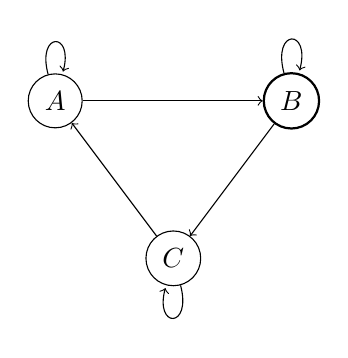
\begin{tikzpicture}
			\node (a)[circle, draw] at (0,0) {$ A $};
			\node (b)[circle, draw, thick] at (3,0) {$ B $};
			\node (c)[circle, draw] at (1.5,-2) {$ C $};
			\draw [->](a)edge (b);
			\draw [->](b)edge (c);
			\draw [->](c)edge (a);

			\draw [-latex](b)edge[loop above] (b);
			\draw [-latex](a)edge[loop above]  (a);
			\draw [-latex](c)edge[loop below]  (c);
		\end{tikzpicture}
	\end{center}
\end{minipage}
%
\begin{minipage}[t]{0.48\textwidth}
	\begin{center}
		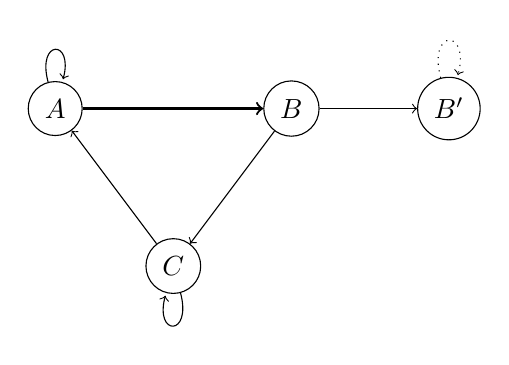
\begin{tikzpicture}
			\node (a)[circle, draw] at (0,0) {$ A $};
			\node (b)[circle, draw] at (3,0) {$ B $};
			\node (c)[circle, draw] at (1.5,-2) {$ C $};
			\node (b1)[circle, draw] at (5,0) {$ B' $};
			\draw [->, thick](a)edge (b);
			\draw [->](b)edge (c);
			\draw [->](b)edge (b1);
			\draw [->](c)edge (a);

			\draw [-latex, dotted](b1)edge[loop above]  (b1);
			\draw [-latex](a)edge[loop above]  (a);
			\draw [-latex](c)edge[loop below]  (c);
		\end{tikzpicture}
	\end{center}
\end{minipage}
\vskip3mm
Il self loop di $ B' $ è tratteggiato in quanto è vero che $ B' $ referenzia $ B' $ per forza, però è anche vero che non sarà mai una ricorsione sinistra, quindi non va considerata
\subsubsection{Esempio 1}
\begin{minipage}[c]{0.48\textwidth}
	\begin{align*}
		E & \rightarrow E + T \mid T       \\
		T & \rightarrow T * F \mid F       \\
		F & \rightarrow (E) \mid \text{id}
	\end{align*}

\end{minipage}
%
\begin{minipage}[c]{0.48\textwidth}
	\begin{center}
		\begin{tikzpicture}[scale=2.5]
			\node (e)[circle, draw] at (0,0) {$ E $};
			\node (t)[circle, draw] at (3,0) {$ T $};
			\node (f)[circle, draw] at (1.5,-2) {$ F $};

			\draw [->, bend left = 10](e)to node[midway, above]{$ E \rightarrow T $}(t);
			\draw [->, bend right = 10, dotted](e)to node[midway, below, opacity=0.2]{$ E \rightarrow E + T $}(t);

			\draw [->, bend left = 10](t)to node[midway, right]{$ T \rightarrow F $}(f);
			\draw [->, bend right, dotted](t)to node[midway, left, opacity=0.2]{$ T \rightarrow T * F $}(f);

			\draw [->, bend left, dotted](f)to node[midway, left, opacity=0.2]{$ F \rightarrow \left(E\right) $}(e);


			\draw [-latex](e)edge[loop above] node [midway, above]{$ E \rightarrow E + T $}  (e);
			\draw [-latex](t)edge[loop above] node [midway, above]{$ T \rightarrow T * F $} (t);
		\end{tikzpicture}
	\end{center}
\end{minipage}
\vskip3mm
Come si vede chiaramente nel grafico, ci sono solo left recursione \textit{immediate}, dunque posso direttamente semplificarle:
\begin{itemize}
	\item $ E \rightarrow E + T \mid T $ diventa:
	      \begin{align*}
		      E  & \rightarrow T E'            \\
		      E' & \rightarrow +TE' | \epsilon
	      \end{align*}
	\item $ T \rightarrow  T * F | F $ diventa:
	      \begin{align*}
		      T  & \rightarrow F T'   \\
		      T' & \rightarrow * F T' \\
	      \end{align*}
\end{itemize}
Quindi ottengo:
\begin{align*}
	E  & \rightarrow TE'                \\
	E' & \rightarrow +TE' \mid \epsilon \\
	T  & \rightarrow FT'                \\
	T' & \rightarrow *FT' \mid \epsilon \\
	F  & \rightarrow (E) \mid \text{id}
\end{align*}

\subsubsection{Esempio 2}
\begin{align*}
	E & \rightarrow E + E \mid E * E \mid (E) \mid \text{id}
\end{align*}

Qui chiaramente non posso avere cicli \textit{non} elementari, dunque procediamo direttamente con l'eliminazione, ottenendo:
\begin{align*}
	E  & \rightarrow (E)E' \mid \text{id}E'       \\
	E' & \rightarrow +EE' \mid *EE' \mid \epsilon
\end{align*}
Si noti però che non è comunque una grammatica LL(1), in quanto partendo da $ E' $, posso ottenere $ + $ tramite
\begin{enumerate}
	\item $ E' \rightarrow +E E' $
	\item $ E' \rightarrow \epsilon  $
\end{enumerate}

abbiamo un risultato importante:
\begin{center}
	Una grammatica non left recursive non è necessariamente LL(1). Allo stesso modo non è garantito che la grammatica non sia ambigua
\end{center}
\subsection{Fattorizzazione sinistra}
Se una grammatica contiene due produzioni i cui body hanno lo stesso prefisso (iniziano per una serie di caratteri uguali), allora per forza di cose la grammatica non e LL(1). Posso però fattorizzare
\begin{definizione}{Fattorizzazione a sinistra}
	La fattorizzazione a sinistra consiste nel delayare quanto possibile la scelta della parte che contraddistingue due produzioni che condividono un prefisso nel body. Ad esempio:
	\[
		S \rightarrow \alpha \beta_1 \mid \alpha \beta_2 \mid \gamma
	\]
	può essere fattorizzata a sinistra in:
	\begin{align*}
		S  & \rightarrow \alpha S' \mid \gamma \\
		S' & \rightarrow \beta_1 \mid \beta_2
	\end{align*}
\end{definizione}
\subsection{Conclusioni}
\begin{itemize}
	\item No left-recursive grammar is LL(1)
	\item No grammar that can be left-factorized is LL(1)
	\item No ambiguous grammar is LL(1)
\end{itemize}
\begin{teorema}{Condizioni LL(1)}
	$\mathcal{G}$ è LL(1) se e solo se per le produzioni $A \rightarrow \alpha \mid \beta$ si ha:

	\begin{itemize}
		\item $\text{first}(\alpha) \cap \text{first}(\beta) = \emptyset$
		\item Se $\epsilon \in \text{first}(\alpha)$ allora $\text{first}(\beta) \cap \text{follow}(A) = \emptyset$
		\item Se $\epsilon \in \text{first}(\beta)$ allora $\text{first}(\alpha) \cap \text{follow}(A) = \emptyset$
	\end{itemize}
\end{teorema}
Intuitivamente, basta costruire la tabella come in sezione \ref{parsing table} e verificare che non ci siano celle con più produzioni canidate
\section{Linguaggi regolari}
Un linguaggio regolare ha una definizione molto semplice:
\begin{definizione}{Linguaggio regolare}
	Un linguaggio regolare è un linguaggio libero in cui ogni produzione ha la forma:
	\begin{itemize}
		\item $ A \rightarrow aA $
		\item $ A \rightarrow a $
		\item $ A \rightarrow \epsilon $
	\end{itemize}
\end{definizione}
Un'espressione regolare è definita per induzione:
\begin{definizione}{Espressione regolare}
	Dato un alfabeto $ \mathcal{A} $,  un'espressione regolare è definita per induzione:
	\begin{itemize}
		\item Caso \textit{base}
		      \begin{itemize}
			      \item Ogni $ a \in \mathcal{A} \cup \epsilon  $ è un'espressione regolare
		      \end{itemize}

		\item Passo \textit{induttivo}. Siano $ r_1 $ e $ r_2 $ due espresioni regolari, allora:
		      \begin{itemize}
			      \item \textit{Alternamento} $ r_1 \mid r_2 $ è un'espressione regolare
			      \item \textit{Concatenazione} $ r_1 r_2 $ è un'espressione regolare
			      \item \textit{Kleene start} $ r^{*} $ ($ r $) ripetuta 0 o più volte è un'espressione regolare
			      \item \textit{Parentesi} $ \left(r_1\right) $ è un'espressione regolare
		      \end{itemize}
	\end{itemize}
\end{definizione}
Nota che la precedenza degli operatori è, partendo dalla più alta
\begin{itemize}
	\item Kleen star
	\item Concatenazione
	\item Alternamento
\end{itemize}
Quindi $ \left(a \mid bc ^{*}\right) $ è equivalente a $ \left(a \mid \left(b \left(c^{*}\right)\right)\right) $
\subsection{Automa non deteministico a stati finiti}
\begin{definizione}{Automa non deteministico a stati finiti}
	Un \textit{automa non deterministico a stati finiti} è una tupla $ \left(\mathcal{S}, \mathcal{A}, \text{move}_n, \mathcal{F}\right) $, dove
	\begin{itemize}
		\item $S$ è un insieme di stati.
		\item $A$ è un alfabeto con $\epsilon \notin A$.
		\item $s_0 \in S$ è lo stato iniziale.
		\item $F \subseteq S$ è l'insieme degli stati finali (o accettanti).
		\item $\text{move}_n : S \times (A \cup \{\epsilon\}) \to 2^S$ è la funzione di transizione.
	\end{itemize}
\end{definizione}\label{nondeterministic automata}
Questo automa può essere rappresentato in maniera conveniente con un grafo dove:
\begin{itemize}
	\item $ \mathcal{S} $ sono i nodi
	\item $ \text{move}_n $ sono gli archi, i cui "pesi" sono dati da lettere $ \in \mathcal{A} $
\end{itemize}
\begin{center}
	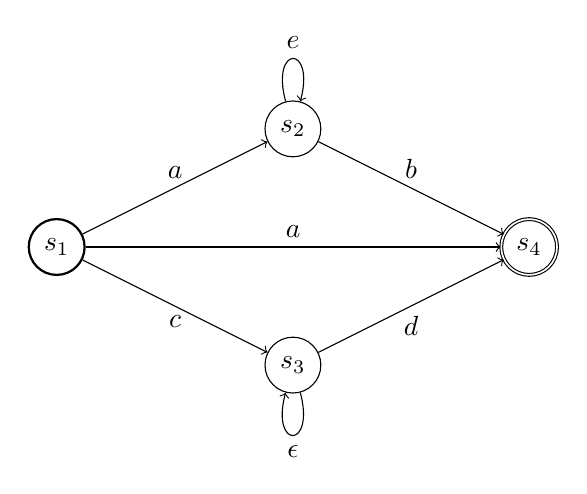
\begin{tikzpicture}[scale = 1.5]
		\node (s1)[draw, circle,thick] at(0,0)  {$ s_1 $};
		\node (s2)[draw, circle] at(2,1)  {$ s_2 $};
		\node (s3)[draw, circle] at(2,-1)  {$ s_3 $};
		\node (s4)[draw, circle, double] at(4,0)  {$ s_4 $};
		\draw [->](s1)--(s2) node[midway, above]{$ a $};
		\draw [->](s2)--(s4) node[midway, above] {$ b $};
		\draw [->](s1)--(s3) node[midway, below] {$ c $};
		\draw [->](s3)--(s4) node[midway, below] {$ d $};
		\draw [->](s1)--(s4) node[midway, above] {$ a $};
		\draw [->](s2)to[loop above] node[midway, above] {$ e $} (s2) ;
		\draw [->](s3)to[loop below] node[midway, below] {$ \epsilon $} (s3) ;
	\end{tikzpicture}
\end{center}
Nota che la funzione di transizione non è proprio ciò che ci si aspetta. Non è una matrice $ n \times n $ in cui se esiste un arco di peso $ a $ fra $ i $ e $ j $ è rappresentato mettendo $ m\left[i\right]\left[j\right] = a $. Qui la matrice ha questa forma:
\begin{center}
	\begin{tabular}{c | c c c c c c}
		\toprule
		        & $ \epsilon  $          & $ a $                       & $ b $                   & $ c $                  & $ d $                   & $ e $                   \\
		\midrule
		$ s_1 $ & $ \emptyset  $         & $ \left\{S_2, S_4\right\} $ & $ \emptyset  $          & $ \left\{S_3\right\} $ & $ \emptyset  $          & $ \emptyset  $          \\
		$ s_2 $ & $ \emptyset  $         & $ \emptyset  $              & $ \left\{S_4\right\}  $ & $ \emptyset  $         & $ \emptyset  $          & $ \left\{S_2\right\}  $ \\
		$ s_3 $ & $ \left\{S_3\right\} $ & $ \emptyset  $              & $ \emptyset  $          & $ \emptyset  $         & $ \left\{s_4\right\}  $ & $ \emptyset  $          \\
		$ s_4 $ & $ \emptyset  $         & $ \emptyset  $              & $ \emptyset  $          & $ \emptyset  $         & $ \emptyset  $          & $ \emptyset  $          \\
		\bottomrule
	\end{tabular}
\end{center}
\subsection{Construzione di Thompson}
Dato un linguaggio regolare, possono costruire un automata che riconosce il suddetto linguaggio. Posso crearlo sfruttando la definizione induttiva di un linguaggio regolare. Ho componenti base per rapprdentare gli operatori:

\begin{center}
	\begin{tikzpicture}[
			scale=0.9,
			node distance=0.5cm,
			state/.style={draw, circle, minimum size=0.4cm},
			final state/.style={draw, circle, double, minimum size=0.4cm},
			gray ellipse/.style={draw, ellipse, fill=mutedblue!50, fill opacity=0.6, text opacity=1, minimum width=2cm, minimum height=1cm}
		]

		% Prima riga: r = r₁ | r₂
		\node at (-2, 3) {$r = r_1 | r_2$};

		\node[state, fill=white] (alt_init) at (0, 3) {};
		\draw[<-] (alt_init) -- +(-0.5, 0);
		\node[final state, fill=white] (alt_final) at (5, 3) {};

		\node[gray ellipse] (alt_r1) at (2.5, 3.8) {$N(r_1)$};
		\node[state, fill=white] (alt_r1_start) at (1.5, 3.8) {};
		\node[state, fill=white] (alt_r1_end) at (3.5, 3.8) {};

		\node[gray ellipse] (alt_r2) at (2.5, 2.2) {$N(r_2)$};
		\node[state, fill=white] (alt_r2_start) at (1.5, 2.2) {};
		\node[state, fill=white] (alt_r2_end) at (3.5, 2.2) {};

		\draw[->] (alt_init) -- (alt_r1_start) node[midway, above] {$\epsilon$};
		\draw[->] (alt_init) -- (alt_r2_start) node[midway, below] {$\epsilon$};
		\draw[->] (alt_r1_end) -- (alt_final) node[midway, above] {$\epsilon$};
		\draw[->] (alt_r2_end) -- (alt_final) node[midway, below] {$\epsilon$};

		% Seconda riga: r = r₁r₂
		\node at (-2, 0) {$r = r_1 r_2$};

		\node[state, fill=white] (cat_init) at (0.5, 0) {};
		\draw[<-] (cat_init) -- +(-0.5, 0);
		\node[final state, fill=white] (cat_final) at (4.5, 0) {};

		\node[gray ellipse] (cat_r1) at (1.5, 0) {$N(r_1)$};
		\node[gray ellipse] (cat_r2) at (3.5, 0) {$N(r_2)$};
		\node[state, fill=white] (cat_mid) at (2.5, 0) {};

		\node[final state, fill=white] (cat_final) at (4.5, 0) {};
		\node[state, fill=white] (cat_init) at (0.5, 0) {};

		% Terza riga: r = r₁*
		\node at (-2, -3) {$r = r_1^*$};

		\node[state, fill=white] (star_init) at (0, -3) {};
		\draw[<-] (star_init) -- +(-0.5, 0);
		\node[final state, fill=white] (star_final) at (5, -3) {};

		\node[gray ellipse] (star_r1) at (2.5, -3) {$N(r_1)$};
		\node[state, fill=white] (star_r1_start) at (1.5, -3) {};
		\node[state, fill=white] (star_r1_end) at (3.5, -3) {};

		\draw[->] (star_init) -- (star_r1_start) node[midway, above] {$\epsilon$};
		\draw[->] (star_r1_end) -- (star_final) node[midway, above] {$\epsilon$};
		\draw[->] (star_init) to[bend left=45] node[midway, above] {$\epsilon$} (star_final);
		\draw[->] (star_r1_end) to[out = -90, in = -90] node[midway, below] {$\epsilon$} (star_r1_start);

		% Quarta riga: r = (r₁)
		\node at (-2, -6) {$r = (r_1)$};

		\node[gray ellipse] (paren_r1) at (2.5, -6) {$N(r_1)$};
		\node[final state, fill=white] (paren_end) at (3.5, -6) {};
		\node[state, fill=white] (paren_start) at (1.5, -6) {};
		\draw[<-] (paren_start) -- +(-0.5, 0);

	\end{tikzpicture}
\end{center}

% \subsubsection*{Elemento base}
% \begin{center}
% 	\begin{tikzpicture}
% 		\node (a)[draw, circle, thick] at (0,0) {};
% 		\node (b)[draw, circle, double] at (2,0) {};
% 		\draw [->](a)-- node[midway, above]{$ a $}(b);
% 		\draw [<-](a)--++(-0.5, 0);
% 	\end{tikzpicture}
% \end{center}
%
% \subsubsection*{Alternamento}
% \begin{center}
% 	\begin{tikzpicture}[scale = 1.5]
% 		% Label at the top
% 		\node at (1.5,2) {$r=r_1|r_2$};
%
% 		% Main nodes
% 		\node (init) [draw, circle, thick] at (0,0) {};
% 		\node (final) [draw, circle, double ] at (5,0) {};
% 		\draw [<-](init)--++(-0.5, 0);
%
% 		% Upper path (r1)
% 		\node (r1) [draw, ellipse, fill=gray!30, minimum width=2.5cm, minimum height=1.2cm] at (2.5,1) {$N(r_1)$};
% 		\node (r1start) [draw, circle,  fill=white, minimum size=0.4cm] at (1.8,1) {};
% 		\node (r1end) [draw, circle,  fill=white, minimum size=0.4cm] at (3.2,1) {};
%
% 		% Lower path (r2)
% 		\node (r2) [draw, ellipse, fill=gray!30, minimum width=2.5cm, minimum height=1.2cm] at (2.5,-1) {$N(r_2)$};
% 		\node (r2start) [draw, circle,  fill=white, minimum size=0.4cm] at (1.8,-1) {};
% 		\node (r2end) [draw, circle,    fill=white, minimum size=0.4cm] at (3.2,-1) {};
%
% 		% Connections for upper path
% 		\draw [->] (init) -- (r1start) node[midway, above] {$\epsilon$};
% 		\draw [->] (r1end) -- (final) node[midway, above] {$\epsilon$};
%
% 		% Connections for lower path
% 		\draw [->] (init) -- (r2start) node[midway, below] {$\epsilon$};
% 		\draw [->] (r2end) -- (final) node[midway, below] {$\epsilon$};
% 	\end{tikzpicture}
% \end{center}
% \subsubsection*{Concatenazione}
% \begin{tikzpicture}[scale = 2]
%
% 	% Regions for r1 and r2
% 	\pgfdeclarelayer{background}
% 	\pgfdeclarelayer{foreground}
% 	\pgfsetlayers{background,main,foreground}
%
% 	\begin{pgfonlayer}{foreground}
% 		\node (a)[draw, thick, circle, fill=white, inner sep = 0.3cm] at (-1.5,0)  {};
% 		\node (b)[draw, circle, fill=white, inner sep = 0.3cm] at (0,0)  {};
% 		\node (c)[draw, double, circle, fill=white, inner sep = 0.3cm] at (1.5,0)  {};
% 		\draw [<-](a)--++(-0.5, 0);
% 	\end{pgfonlayer}
% 	\begin{pgfonlayer}{background}
% 		\node (n1)[inner sep =0, fit = (a) (b), draw, ellipse, fill=gray, fill opacity=0.4, text opacity = 1]  {\contour{white}{$ N\left(r_1\right) $}};
% 		\node (n1)[inner sep =0, fit = (b) (c), draw, ellipse, fill=gray, fill opacity=0.4, text opacity = 1]  {\contour{white}{$ N\left(r_2\right) $}};
% 	\end{pgfonlayer}
% \end{tikzpicture}
\subsection{Simulazione}
La simulazione è il processo che dato un automa ci permette di verificare se una parola appartiene al linguaggio generato da esso
\begin{definizione}{$ \epsilon$ - chiusura}
	Dato un insieme di stati di un automa, la $ \epsilon $ chiusura si uno stato $ S $ è l'insieme di stati raggiungibili da $ S $ tramite soli archi $ \epsilon $
\end{definizione}

Possiamo sfruttare il concetto di $ \epsilon  $- chiusura per verificare se una parola appartiene al linguaggio generato da un automa.
\begin{itemize}
	\item Teniamo traccia in una struttura \verb|states| gli stati "buoni" in questo momento
	\item  Inizialmente, \verb|states| contiene la $ \epsilon  $- chiusura dello stato iniziale
	\item Per ogni carattere $ c $, \verb|states| diventa la $ \epsilon  $- chiusura di \textit{tutti gli stati raggiungibili da states tramite soli archi $ c $}
	\item Si itera finchè non si arriva a fine parola
	\item Se in \verb|states| ho almeno uno stato finale significa che $ w \in L $, altrimenti no
\end{itemize}
\subsection{Automa deterministico a stati finiti}
\begin{definizione}{Automa deterministico a stati finiti}
	Un \textit{automa deterministico a stati finiti} è una tupla $ \left(\mathcal{S}, \mathcal{A}, \text{move}_n, \mathcal{F}\right) $, dove
	\begin{itemize}
		\item $S$ è un insieme di stati.
		\item $A$ è un alfabeto con $\epsilon \notin A$.
		\item $s_0 \in S$ è lo stato iniziale.
		\item $F \subseteq S$ è l'insieme degli stati finali (o accettanti).
		\item $\text{move}_n : S \times A  \to S$ è la funzione di transizione.
	\end{itemize}
\end{definizione}
La differenza rispetto all'\hyperref[nondeterministic automata]{automa deterministico}, sta nel fatto che
\begin{itemize}
	\item Non vi sono $ \epsilon  $- transizioni
	\item Ogni nodo ha \textit{al più} un arco uscente pero ogni $ a \in \mathcal{A} $
\end{itemize}
Questo perché
\begin{itemize}
	\item \sfblue{NFA}: $(S, A, \text{move}_n, s_0, F)$
	      \begin{itemize}
		      \item[] \textit{dove} $\text{move}_n : S \times (A \cup \{\epsilon\}) \to 2^S$
	      \end{itemize}

	\item \sfblue{DFA}: $(S, A, \text{move}_d, s_0, F)$
	      \begin{itemize}
		      \item[] \textit{dove} $\text{move}_d : S \times A \to S$
	      \end{itemize}
\end{itemize}
Nota che dato un nodo $ S $ avendo un solo arco per ogni $ a \in \mathcal{A} $, è molto facile controllare se $ w \in L $. Basta \textit{seguire} il perscorso, che è unico
\subsubsection{Completamento funzione DFA}\label{completamento funzione di transizione}
Spesso torna utile avere una funzione completa in un DFA. Per fortuna è sempre possibile prendere una funzione di transizione \textit{parziale} e completarla come segue:
\begin{itemize}
	\item Introduco nuovo nodo \verb|sink|
	\item Per ogni nodo $ n $ a cui manca un arco uscente per una lerrea $ c $ dell'alfabeto, aggiungo arco $ \left(n, \text{\ttfamily sink}\right)_{c} $
	\item Per ogni lettera dell'alfabeto, aggiungo arco $ \left(\text{\ttfamily sink}, \text{\ttfamily sink}\right)_c $
\end{itemize}

\subsubsection{Conversione da NFA a DFA}
L'algoritmo è lento in culo e tedioso, però funziona come segue:
\begin{itemize}
	\item Prendi la $\epsilon$-chiusura di $ S_0 $ e la chiamo $ T $
	\item Per ogni lettera dell'alfabeto $ x $, devo vedere in quali nodi mi possa portare. Dunque considero l'insieme di nodi raggiungibili da un qualsiasi nodo di $ T $ con una $ x $- transizione
	\item Calcolo la $ \epsilon $-chiusura di questo insieme. Se l'insieme è gia stato ottenuto, aggiungo un arco $ x $ da $ T $ all'insieme già ottenuto. Altrimenti ne creo un'altro e aggiungo l'arco
	\item Nota che gli insiemi non devono essere per forza disgiunti, anzi, è raro che lo siano
\end{itemize}
\subsubsection{Minimizzazione DFA}
L'idea di base si basa sul concetto di equivalenza di stati:
\begin{definizione}{Equivalenza di due stati}
	Dadi due stati $ s $ e $ t $ di un DFA $ D $, questi si dicono equivalenti se importando il nodo di partenza su di uno o sull'altro ottengo lo  stesso linguaggio. Formalmente:
	\[
		\mathcal{L}_D \left(s\right) =     \mathcal{L}_D \left(t\right)
	\]
\end{definizione}
L'idea è quindi quella di partizionare il grafo in \textit{gruppi di stati equivalenti}. L'algoritmo si basa sulla seguente proprietà:
\begin{center}
	Se due stati $ s $ e $ t $ sono equivalenti, allora non possono esistere $ \alpha $-archi che partano da $ s $ e $ t $ e vadano in due gruppi diversi
\end{center}
Questo perché per come costruiamo i gruppi, sicuramente se due nodi stanno in due gruppi diversi non sono equivalenti. Dunque per forza se faccio
\begin{itemize}
	\item Parto da $ s $ e vado con un arco $ a $ in $ B_1 $:
	      \[
		      s \rightarrow_a B_1 \quad \text{ ottengo } a \mathcal{L}\left(B_1\right)
	      \]
	\item Parto da $ t $ e vado con un arco $ a $ in $ B_2 $:
	      \[
		      t \rightarrow_a B_2 \quad \text{ ottengo } a \mathcal{L}\left(B_2\right)
	      \]
\end{itemize}
Siccome, per come costruiamo i gruppi $ \mathcal{L}\left(B_1\right) \neq \mathcal{L}\left(B_2\right) $, per forza si cose gli stati $ s $ e $ t $ \textit{non} sono equivalenti
La procedura di minimizzazione procede così:
\begin{itemize}
	\item Completo la funzione di transizione del DFA, come descritto in sezione \ref{completamento funzione di transizione}
	\item Partiziono i nodi dell'automata in due insiemi:
	      \begin{itemize}
		      \item $ F $: gli stati finali
		      \item $ S - F $: gli stati non finali
	      \end{itemize}
	\item Se esistono due nodi $ s $ e $ t $ che hanno delle $ \alpha  $ - transizioni in gruppi diversi, allora posso spezzare il gruppo corrente
	\item Supponendo di aver trovare $ s $ e $ t $ che puntano in due gruppi diversi $ B_1 $ e $ B_2 $ tramite $ \alpha $- transizione, allora posso dividere il gruppo corrente $ B $ in due
	      \begin{itemize}
		      \item I nodi che puntano in $ B_1 $
		      \item I nodi che puntano in $ B_2 $
	      \end{itemize}
	\item Procedo ricorsivamente finchè possibile. Posso raggruppare in un singolo nodi i gruppi che non possono essere splittati ulteriormente
\end{itemize}
\subsubsection{Numero stati di un DFA}
Sappiamo che fare parsin tramite un NFA è meno efficiente rispetto che tramite DFA. Tuttavia, non è tutto oro ciò che luccica
\begin{teorema}{Numero stati di un DFA}
	Per ogni NFA con $ n+1 $ stati esiste un DFA corrispondente che ha almeno $ 2^{n} $ stati e una funzione di transizione totale
\end{teorema}
Questo equivale a dire che nel caso pessimo, convertendo un NFA con $ n $ nodi otteniamo un DFA con $ 2^{n} $ nodi
\sfblue{Dimostrazione:}
Considero linguaggio dato da
\[
	\mathcal{L} = \mathcal{L}\left(\left(a \mid b\right)^{*} a \left(a | b\right)^{n-1}\right)
\]
\begin{center}
	\begin{tikzpicture}[
			auto,
			state/.style={circle, draw, inner sep=8pt},
		]

		% States
		\node[state, thick] (q0) {};
		\node[state, right=of q0] (q1) {};
		\node[state, right=of q1] (q2) {};
		\node[state, right=of q2] (q3) {};
		\node[state, right= of q3, double] (q4) {};

		% Transitions
		\draw[-latex] (q0) edge[loop above] node{a,b} (q0);
		\draw[-latex] (q0) edge node{a} (q1);
		\draw[-latex] (q1) edge node{a,b} (q2);
		\draw[-latex] (q2) edge node{a,b} (q3);
		\draw[-latex, dashed] (q3) edge node{a,b} (q4);

	\end{tikzpicture}
\end{center}
Ora consideriamo due parole diverse di lunghezza $ n $: $ w_1 $ e $ w_2 $. Dato che le parole sono diverse, allora esiste un indice $ k $ al quale una sarà $ a $ e l'altra $ b $. Senza perdita di generalità assumiamo che
\begin{align*}
	w_1 = \underbracket[0.1ex]{\ldots }_{k-1} a \underbracket[0.1ex]{\ldots}_{n - k} &  &
	w_1 = \underbracket[0.1ex]{\ldots }_{k-1} b \underbracket[0.1ex]{\ldots}_{n - k}
\end{align*}
Ossia che in posizione $ k $ esima $ w_1 = a $ e $ w_2 =b $. Ora notiamo che
\begin{align*}
	 & w_1 b^{k} \in \mathcal{L}
	 & w_2 b^{k} \not \in \mathcal{L}
\end{align*}
Questo perchè
\begin{align*}
	w_1 b^{k} = \underbracket[0.1ex]{\ldots }_{k-1} a \overbracket[0.1ex]{\underbracket[0.1ex]{\ldots}_{n - k} b^{k}}^{n} &  &
	w_2 b^{k} = \underbracket[0.1ex]{\ldots }_{k-1} b \overbracket[0.1ex]{\underbracket[0.1ex]{\ldots}_{n - k} b^{k}}^{n}
\end{align*}
Quindi la seconda non è il $ \mathcal{L} $ in quanto non finisce per a seguita da $ n $ caratteri. Ora ragioniamo così:
\begin{itemize}
	\item Due parole distinte non possono terminare nello stesso stato. Questo sarebbe assurdo in quanto abbiamo dimostrato che una è accettata dal linguaggio e una non lo è. Se finissero sullo stesso stato dovrebbero essere entrambe accettate oppure non accettate
	\item Siccome su $ \left\{a, b\right\} $ esistono $ 2^{k} $ parole distinte, e per ogni parola distinta necessito di almeno uno stato, allora gli stati del DFA sono almeno $ 2^{n} $
\end{itemize}
\subsection{Pumping lemma per linguaggi regolari}
\begin{teorema}{Pumping lemma per linguaggi regolari}
	Dato un linguaggio regolare $ \mathcal{L}\left(\mathcal{G}\right) $, allora:
	\begin{itemize}
		\item Dato $ p \ge 0 $
		\item $ \forall z \text{ t.c. } \left|z\right| > p $ valgono le seguenti condizioni:
		\item Allora esiste un \textit{"unpacking"} di $ z $, ossia $ z = uvw $ tale per cui
		      \begin{itemize}
			      \item $ \left|vw\right| \le p $
			      \item $ \left|v\right| > 0$
			      \item $ \forall i \in \N \quad u v^{i} w  \in \mathcal{L}\left(\mathcal{G}\right) $
		      \end{itemize}
	\end{itemize}
\end{teorema}
\sfblue{Dimostrazione:} considero l'automa DFA relativo a $ \mathcal{L} $
\begin{itemize}
	\item Scelgo $ p = \left|S\right|$ dove $ \left|S\right| $ è il numero di stati dell'automa
	\item Noto che ogni parola $ w $ con $ \left|w\right| > p $ è formata da un path nell'automa che ha almeno un nodo che viene visitato \textit{due volte}
	\item Questo garantisce che il path che genera la parola $ w $ convenga un ciclo. Chiamando il nodo che viene visitato due volte $ s $, allora il path che genera $ w $ è
	      \[
		      a_1 \ldots s\; a_i\; \ldots  a_{j}\; s \ldots a_z
	      \]
	      dunque posso eseguire l'unpacking come segue:
	      \begin{align*}
		      u & = a_1 \ldots s           \\
		      v & = s\; a_i \ldots a_j\; s \\
		      w & = s \ldots a_z           \\
	      \end{align*}
\end{itemize}
Dunque posso eseguire il pumping percorrendo il ciclo all'infinito



\section{Bottom up parsing}
\begin{align*}
	S & \rightarrow xS \mid yA \\
	A & \rightarrow a \mid aA  \\
\end{align*}
L'idea è di costruire un automa che matchi una qualsiasi espansione parziale questo alfabeto. Ad esempio, creiamo un automa che matchi sia $ xxyaa $, ma anche $ xxyA $.
\vskip3mm
Innanzitutto, costruiamo un automa che matchi ogni produzione base della grammatica. Questo è facile da ottenere
\begin{center}
	\begin{tikzpicture}
		\node (1)[draw, circle, thick] at (0,0)  {};
		\node (2)[draw, circle, right of = 1, double] {};

		\node (3)[draw, circle, below of = 1] {};
		\node (4)[draw, circle, right of = 3] {};
		\node (5)[draw, circle, right of = 4, double] {};

		\node (6)[draw, circle, below of = 3] {};
		\node (7)[draw, circle, right of = 6] {};
		\node (8)[draw, circle, right of = 7, double] {};

		\node (9)[draw, circle, below of = 6, shift={(0,-0.5)}] {};
		\node (10)[draw, circle, right of = 9, double] {};

		\node (11)[draw, circle, below of = 9] {};
		\node (12)[draw, circle, right of = 11] {};
		\node (13)[draw, circle, right of = 12, double] {};

		\node (14)[draw, circle, below of = 11] {};
		\node (15)[draw, circle, right of = 14, double] {};

		\draw [->](1) to node (l1)[midway, above] {$S$}(2);

		\draw [->](3) to node [midway, above] {$x$}(4);
		\draw [->](4) to node [midway, above] {$S$}(5);

		\draw [->](6) to node [midway, above] {$y$}(7);
		\draw [->](7) to node [midway, above] {$A$}(8);


		\draw [->](9) to node (l2) [midway, above] {$A$}(10);

		\draw [->](11) to node [midway, above] {$a$}(12);
		\draw [->](12) to node [midway, above] {$A$}(13);

		\draw [->](14) to node [midway, above] {$a$}(15);


		\node [fit = (1) (8) (l1), dotted, draw, label={0:{$ S \rightarrow xS \mid yA $}}]  {};

		\node [fit = (9) (13) (15) (l2), dotted, draw,  label={0:{$ A \rightarrow a \mid aA $}}]  {};
	\end{tikzpicture}

\end{center}
Dopodichè bisogna ragionare nel seguente modo. Se siamo in uno stato qualsiasi, possiamo matchare come prossima cosa sia un simbolo già matchato (es $ S $), sia una sua qualsiasi espansione (es $ xS $ o $ yA $). Dunque devo aggiungere archi secondo questa precisa logica

\begin{center}
	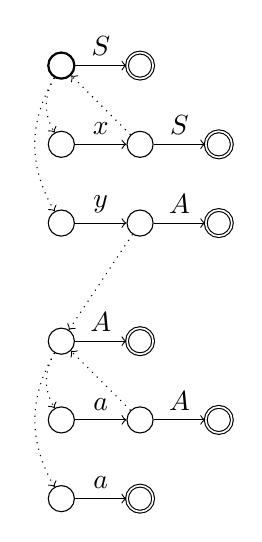
\begin{tikzpicture}
		\node (1)[draw, circle, thick] at (0,0)  {};
		\node (2)[draw, circle, right of = 1, double] {};

		\node (3)[draw, circle, below of = 1] {};
		\node (4)[draw, circle, right of = 3] {};
		\node (5)[draw, circle, right of = 4, double] {};

		\node (6)[draw, circle, below of = 3] {};
		\node (7)[draw, circle, right of = 6] {};
		\node (8)[draw, circle, right of = 7, double] {};

		\node (9)[draw, circle, below of = 6, shift={(0,-0.5)}] {};
		\node (10)[draw, circle, right of = 9, double] {};

		\node (11)[draw, circle, below of = 9] {};
		\node (12)[draw, circle, right of = 11] {};
		\node (13)[draw, circle, right of = 12, double] {};

		\node (14)[draw, circle, below of = 11] {};
		\node (15)[draw, circle, right of = 14, double] {};

		\draw [->](1) to node (l1)[midway, above] {$S$}(2);

		\draw [->](3) to node [midway, above] {$x$}(4);
		\draw [->](4) to node [midway, above] {$S$}(5);

		\draw [->](6) to node [midway, above] {$y$}(7);
		\draw [->](7) to node [midway, above] {$A$}(8);


		\draw [->](9) to node (l2) [midway, above] {$A$}(10);

		\draw [->](11) to node [midway, above] {$a$}(12);
		\draw [->](12) to node [midway, above] {$A$}(13);

		\draw [->](14) to node [midway, above] {$a$}(15);


		% \node [fit = (1) (8) (l1), dotted, draw, label={0:{$ S \rightarrow xS \mid yA $}}]  {};
		% \node [fit = (9) (13) (15) (l2), dotted, draw,  label={0:{$ A \rightarrow a \mid aA $}}]  {};


		\draw [dotted,->](4) to (1);
		\draw [dotted,->, bend right](1) to (3);
		\draw [dotted,->, bend right](1) to (6);

		\draw [dotted,->](7) to (9);
		\draw [dotted,->, bend right](9) to (11);
		\draw [dotted,->, bend right](9) to (14);

		\draw [dotted,-> ](12) to (9);
	\end{tikzpicture}
\end{center}
L'idea è proprio che se sono su un nodo qualsiasi, posso aspettarmi che dopo venga il simbolo già ridotto ($ S, A $), oppure qualsiasi stringa derivante da una sua espansione. Collego quindi ogni arco $ S_1 \rightarrow_{\text{non terminale}} S_2  $ ad ogni "sotto automa" che rappresenta una produzione basilare. Nota che si generano archi inutili
\subsection{LR(0) items}
Per capire bene come definire un automa di parsing lr(0), è necessario chiarire il concetto di \textit{LR(0)-item}.
\vskip3mm
L'idea di base è che nel parsing bottom up, un parsers cerca di matchare una porzione di una stringa come espansione di un driver. Le informazioni riguardo cosa sta cercando di matchare con cosa sono contenute in un LR(0)-item.
\begin{definizione}{LR(0) item}
	Un item LR(0) è una produzione nella forma
	\[
		A \rightarrow \alpha \cdot \beta
	\]
	L'item indica che il parser sta cercando di matchare con $ A $ una stringa con forma $ \alpha \beta $. In particolare $ \alpha  $ è già stato matchato, mentre $ \beta $ no
\end{definizione}
\subsubsection{Chiusura di un LR(0) item}
Per la costruzione di un automa LR(0), è necessario definire la chiusura di un LR(0) item. Intuitivamente, la chiusura di un item LR(0) $ A \rightarrow \alpha \cdot \beta  $ è l'insieme di LR(0) items che potrebbe essere necessario matchare \textit{transitivamente} per matchare $ A $
Supponendo di avere
\begin{align*}
	S & \rightarrow Sb \mid Ab \mid s \\
	A & \rightarrow S \mid a
\end{align*}
Se sono in uno stato in cui sto cercando di matchare l'espansione $ S' \rightarrow \cdot S $, allora posso transitivamente star cercando di matchare ogni sottoalbero sinistro:
\vskip3mm
\begin{center}
	\begin{forest}
		for tree={ grow = -90}
		[$ S' $ [S, draw, dotted [Sb, draw, dotted [S]][Ab, draw, dotted[A, draw, dotted [S][a]]][$s$]]]
	\end{forest}
\end{center}
Operativamente per calcolare la chiusura devo:
\begin{itemize}
	\item Per ogni nella forma $ A \rightarrow \alpha \cdot B \beta $, ossia ogni LR(0) item con un \textit{non terminale} immediatamente dopo il pallino
	\item Prendo ogni produzione $ B \rightarrow \gamma $ e aggiungo l'item $ B \rightarrow \cdot \gamma $ alla chiusura se non è già presente
	\item Ripeto fino a saturazione
\end{itemize}
% Partiamo dalla stringa $ abbb $. Siccome vogliamo che l'automa riconosca sia stringhe di terminali, sia occorrenze parzialmente ridotte, avremmo: 
\subsection{Costruzione automa LR(0)} \label{costruzione automa lr0}
L'idea nella costruzione dell'automa LR(0) è quella mettere in ciascun stato un insieme di $ LR\left(0\right) $ items, che indicano tutte le possibili espansioni che il parser sta cercando di matchare nel momento in cui si trova nel nodo corrente. Dunque, formalmente
\begin{itemize}
	\item Partiano calcolando la LR(0)-closure del LR(0) nuovo $ S' \rightarrow \cdot S $. Questo contiene tutto ciò che il parser può star cercando di matchare senza ancora aver matchato nulla
	\item Aggiungo un arco uscente per ogni carattere presente dopo il pallino in qualsiasi LR(0) item del nodo corrente, ad es:
	      \begin{align*}
		      S' & \rightarrow \cdot S               \\
		      S  & \rightarrow \cdot A               \\
		      A  & \rightarrow \cdot \left(AB\right) \\
		      A  & \rightarrow \cdot \left(\right)   \\
	      \end{align*}
	      a sinistra del pallino avrò $ \left\{S,A,(\right\} $. Aggiungo un arco uscrente per ciascun dei seguenti simboli
	\item L'idea è che con un'$ A $-transizione posso arrivare ai nuovi stati, matchando il carattere immediatamente a sinistra del pallino.
	\item Gli LR(0) items tramite cui arrivo al nuovo stato costituiscono il \textit{kernel} del nodo.
	      \begin{center}
		      \begin{tikzpicture}
			      \node (T0)[draw, , label={$T_0$}] at (0,0){
				      $\begin{aligned}
						      S' & \rightarrow \cdot S               \\
						      S  & \rightarrow \cdot A               \\
						      A  & \rightarrow \cdot \left(AB\right) \\
						      A  & \rightarrow \cdot \left(\right)   \\
					      \end{aligned}$
			      };

			      \node (T1)[draw, dotted,  right = of T0, label={$T_1$}] { $ S' \rightarrow S \cdot $};

			      \node (T2)[draw, dotted, left = of T0, , label={$T_2$}] {
				      $\begin{aligned}
						      A & \rightarrow  \left(\cdot \right)   \\
						      A & \rightarrow  \left(\cdot AB\right)
					      \end{aligned}$ };

			      \node (T3)[draw, dotted, below = of T0, label=-90:{$T_3$}] { $ S \rightarrow A \cdot $ };
			      \draw [->](T0)to node[midway, above] {S} (T1);
			      \draw [->](T0)to node[midway, above] {(} (T2);
			      \draw [->](T0)to node[midway, right] {A} (T3);
		      \end{tikzpicture}
	      \end{center}

	\item Ora calcolo la chiusura di ogni nuovo nodo aggiunto ($ T_1, T_2, T_3 $)
	      \begin{center}
		      \begin{tikzpicture}
			      \node (T0)[draw, , label={$T_0$}] at (0,0){
				      $\begin{aligned}
						      S' & \rightarrow \cdot S               \\
						      S  & \rightarrow \cdot A               \\
						      A  & \rightarrow \cdot \left(AB\right) \\
						      A  & \rightarrow \cdot \left(\right)   \\
					      \end{aligned}$
			      };

			      \node (T1)[draw,   right = of T0, label={$T_1$}] { $ S' \rightarrow S \cdot $};

			      \node (T21)[draw,  left = of T0, , label={$T_2$}] {
				      $\begin{aligned}
						      A & \rightarrow  \left(\cdot \right)   \\
						      A & \rightarrow  \left(\cdot AB\right)
					      \end{aligned}$
			      };
			      \node (T22)[draw, dotted, below = 0pt of T21, label=180:closure] {
				      $\begin{aligned}
						      A & \rightarrow  \cdot \left(\right)   \\
						      A & \rightarrow  \cdot \left(AB\right)
					      \end{aligned}$
			      };

			      \node (T3)[draw,  below = of T0, label=-90:{$T_3$}] { $ S \rightarrow A \cdot $ };
			      \draw [->](T0)to node[midway, above] {S} (T1);
			      \draw [->](T0)to node[midway, above] {(} (T21);
			      \draw [->](T0)to node[midway, right] {A} (T3);
		      \end{tikzpicture}
	      \end{center}
\end{itemize}
\subsection{Costruzione tabella di parsing}\label{costruzione tabella parsing lr0}
Una volta costruito un automa come in \ref{costruzione automa lr0}, è necessario costruire la tabella di parsing. Intuitivamente, mettiamo
\begin{itemize}
	\item Su ogni riga: stati dell'automa
	\item Su ogni colonna: lettere alfabeto
\end{itemize}
Riempiamo poi la tabella come segue. \verb|tab[P][Y]| indica che sono nello stato \verb|P| e sto cercando di percorrere l'arco \verb|Y|. Dunque \verb|tab[P][Y]| =
\begin{itemize}
	\item \textit{Shift} se \verb|Y| è terminale, ossia percorro arco $ Y $
	\item \textit{Goto} se \verb|Y| è non terminale, ossia percorro arco $ Y $
	\item \textit{Reduce} in \verb|tab[P][Y]| è contenuto un \textit{reducing item}
	\item \textit{Accept} se in \verb|tab[P][Y]| è contenuto l'\textit{accepting item} ($ S' \rightarrow S\cdot  $)
\end{itemize}
Affinchè la tabella possa essere costruita, non devono esserci celle con entrambi
\begin{itemize}
	\item \textit{Shift-reduce}
	\item \textit{Reduce-reduce}
\end{itemize}
Questo dipende dalla grammatica. Appunto, per definizione, una grammatica è SLR(1) se ciò \textit{NON accade}
\subsection{Algoritmo di parsing}
Una volta costruito un automa come in \ref{costruzione automa lr0}
\begin{itemize}
	\item Inizialmente parto sul nodo $ T_0 $
	\item Tengo traccia del path di nodi visitato in \verb|state_stack|
	\item Tengo traccia del path di nodi visitato in \verb|state_stack|
	\item Tengo traccia della riduzione parziale della parola in \verb|symbol_stack|
	\item Controllo se posso fare un'operazione di \textit{shift/goto}. Se possibile la eseguo
	\item Se approdo in un nodo reduce con forma: $ A \rightarrow \alpha \cdot  $, significa che ho matchato un'espansione. Dunque
	      \begin{itemize}
		      \item Rimuovo $ \left|\alpha\right| $ caratteri da \verb|symbol_stack| e inserisco la loro riduzione $ A $
		      \item Rimuovo $ \left|\alpha\right| $ carattedi da \verb|state_stack|. Avendo matchato $ A $, allora devo ricominciare a matchare dallo stato in cui ho iniziato a matchare $ A $ stesso
	      \end{itemize}
	\item Se approdo in un nodo con \textit{accept}, so di aver matchato l'intera parola
\end{itemize}
Nota che questo algoritmo è leggermente diverso da quello proposto dalla professoressa, in quanto
\begin{itemize}
	\item Nella costruzione della tabella di parsing, la prof inserisce \textit{reduce} $ A \rightarrow \beta $ solo se il carattere che viene dopo appartiene ai follow(A)
	\item La riduzione non avviene direttamente se poi non esiste un arco con il carattere seguente
	\item L'algoritmo non gestisce separatamente i \textit{goto}. Effettivamente i \textit{goto} possono solo avvenire nel momento in cui c'è una riduzione
	\item Inoltre, ogni qualvolta avvenga una riduzione, l'algoritmo "riavvolge" il path (esegue il pop da \verb|symbol_stack| e \verb|state_stack|) viene in automatico eseguito il \textit{goto}. Questo è possibile in quanto:
	      \begin{itemize}
		      \item Se una cella contiene \textit{reduce} $ A \rightarrow \alpha \cdot  $, allora, riavvolgendo approdo necessariamente su una cella con un item $ A \rightarrow \cdot \alpha $
		      \item La produzione $ A \rightarrow \cdot \alpha $ sicuramente non è nel kernel dello stato. Questo perché è nel kernel se è derivata da una transizione (ci sono arrivato tramite arco), e in questo caso le stellina è almeno in seconda posizione.
		      \item Se il nodo è il primo ($ T_0 $), allora c'è la produzione aggiuntiva $ S' \rightarrow S $ che fa da cuscinetto. Non riavvolgerò mai ad un'espansione di $ S' $ un quando l'unico modo sarebbe di riavvolgere dall'\textit{accepting node} ma li l'algoritmo termina
	      \end{itemize}
\end{itemize}

\section{Competenze richieste}
\subsection{Linguaggi liberi}
\subsubsection{Preliminari e lemmas}
\begin{itemize}
	\item Chiusura linguaggi liberi rispetto all'\textit{unione}
	\item Chiusura linguaggi liberi rispetto all'\textit{concatenazione}
	\item Non chiusura linguaggi liberi rispetto all'\textit{intersezione}
	\item Forma normale di \textit{Chomsky} e algoritmo per trasformare linguaggio libero in CNF
\end{itemize}

\subsubsection{Pumping Lemma}
\begin{itemize}
	\item Dimostrazione
	\item Applicazione per dimostrare che un linguaggio \textit{non} è libero
\end{itemize}
\subsubsection{Altro}
\begin{itemize}
	\item Alcuni linguaggi liberi noti (es $ \left\{a^{n}b^{n} \mid n > 0\right\} $)
\end{itemize}

\subsection{Top down parsing}
\subsubsection*{Parsing}
\begin{itemize}
	\item Calcolo $ first\left(\alpha \right) $
	\item Calcolo $ follow\left(\alpha \right) $
	\item Costruzione della tabella di parsing LL(1)
	\item Algoritmo di parsing LL(1)
\end{itemize}

\subsubsection*{Caratteristiche linguaggi LL(1)}
\begin{itemize}
	\item Left recursion e metodi di eliminazione
	\item Fattorizzazione a sinistra
	\item Condizione per cui un linguaggio è LL(1)
\end{itemize}
\subsection{Linguaggi regolari}
\begin{itemize}
	\item Definizione espressione regolare e linguaggio regolare
	\item Definizione automa a stati finiti non deterministico (NFA)
	\item Definizione automa a stati finiti deterministico (DFA)
	\item Costruzione di \textit{Thompson} (analisi complessità e spazio)
	\item Simulazione di un NFA (analisi complessità e spazio)
	\item Completamento funzione di transizione
	\item Subset construction (\textit{convertsione} da NFA a DFA)
	\item Minimizzazione di un DFA (metodo del partizionamento)
	\item \textit{Pumping lemma} per linguaggi regolari
\end{itemize}
\subsection{Bottom up parsing}
\begin{itemize}
	\item LR(0) items e chiusura
	\item Costruzione automa LR(0)
	\item Costruzione tabella di parsing LR(0)
	\item Algoritmo di parsing LR(0)
	\item Risoluzione conflitti
\end{itemize}

\subsection{Syntax Directed Definitions}
\begin{itemize}
	\item Valutazione di un SDD
	\item Grammatiche $ S $ attibuite e grammatiche $ L $ attributite
	\item Valutazione espressioni arimetiche grammatiche LARL(1) (\textit{S attribuite})
	\item Valutazione espressioni arimetiche grammatiche LL(1) (\textit{L atributite})
	\item Valutazione SDD durante il parsing SLR(1)
	\item Casi d'esempio:
	      \begin{itemize}
		      \item Valutazione numeri (binario, ottale, decimale)
		      \item Conversione numeri (\verb|float|, \verb|integers|)
		      \item Creazione \textit{abstract syntax tree}
	      \end{itemize}
\end{itemize}
\subsection{Generazione codice intermedio}
\begin{itemize}
	\item Traduzione di \textit{espressioni aritmetiche}
	\item Traduzione di \textit{control flow} (while, if, not, booleani)
	\item Tecnica del \textit{fall}
	\item Tipizzazione arrays
	\item Accesso ad arrays
\end{itemize}
\section{Collezione di grammatiche e parsing table}

\subsection{Grammatica 1}
% \newcommand{\defineProduction}[1]{}

\def\rOneLabel{R1}
\def\rOneDesc{S \to a A B e}

\def\rTwoLabel{R2}
\def\rTwoDesc{A \to A b c}

\def\rThreeLabel{R3}
\def\rThreeDesc{A \to b}

\def\rFourLabel{R4}
\def\rFourDesc{B \to d}



\begin{align*}
	\rOneLabel  :\;  & \rOneDesc   \\
	\rTwoLabel  :\;  & \rTwoDesc   \\
	\rThreeLabel :\; & \rThreeDesc \\
	\rFourLabel :\;  & \rFourDesc  \\
\end{align*}

\begin{center}

	\begin{tabular}{ccc}
		\toprule
		Symbol & First set & Follow set \\
		\midrule
		S      & a         & \$         \\
		A      & b         & b, d       \\
		B      & d         & e          \\
		\bottomrule
	\end{tabular}
	\vskip3mm

	\begin{table}[H]
		\begin{center}
			\begin{tabular}{c c c c c c c c c c}
				\toprule
				State & $a$          & $b$          & $c$          & $d$          & $e$          & $\$$         & $S$ & $A$ & $B$ \\
				\midrule
				0     & S2           &              &              &              &              &              & 1   &     &     \\
				1     & ACC          & ACC          & ACC          & ACC          & ACC          & ACC          &     &     &     \\
				2     &              & S4           &              &              &              &              &     & 3   &     \\
				3     &              & S6           &              & S7           &              &              &     &     & 5   \\
				4     & \rThreeLabel & \rThreeLabel & \rThreeLabel & \rThreeLabel & \rThreeLabel & \rThreeLabel &     &     &     \\
				5     &              &              &              &              & S8           &              &     &     &     \\
				6     &              &              & S9           &              &              &              &     &     &     \\
				7     & \rFourLabel  & \rFourLabel  & \rFourLabel  & \rFourLabel  & \rFourLabel  & \rFourLabel  &     &     &     \\
				8     & \rOneLabel   & \rOneLabel   & \rOneLabel   & \rOneLabel   & \rOneLabel   & \rOneLabel   &     &     &     \\
				9     & \rTwoLabel   & \rTwoLabel   & \rTwoLabel   & \rTwoLabel   & \rTwoLabel   & \rTwoLabel   &     &     &     \\
				\bottomrule
			\end{tabular}
			\caption{Tabella LR(0) senza pruning}
		\end{center}
	\end{table}


	\begin{table}[H]
		\begin{center}
			\begin{tabular}{c c c c c c c c c c}
				\toprule
				State & $a$ & $b$          & $c$ & $d$          & $e$         & $\$$       & $S$ & $A$ & $B$ \\
				\midrule
				0     & S2  &              &     &              &             &            & 1   &     &     \\
				1     &     &              &     &              &             & ACC        &     &     &     \\
				2     &     & S4           &     &              &             &            &     & 3   &     \\
				3     &     & S6           &     & S7           &             &            &     &     & 5   \\
				4     &     & \rThreeLabel &     & \rThreeLabel &             &            &     &     &     \\
				5     &     &              &     &              & S8          &            &     &     &     \\
				6     &     &              & S9  &              &             &            &     &     &     \\
				7     &     &              &     &              & \rFourLabel &            &     &     &     \\
				8     &     &              &     &              &             & \rOneLabel &     &     &     \\
				9     &     &              &     &              & \rTwoLabel  &            &     &     &     \\
				\bottomrule
			\end{tabular}
			\caption{Tabella LR(0) \textit{con} pruning}
		\end{center}
	\end{table}
\end{center}

\subsection{Grammatica 2}
\href{https://mdaines.github.io/grammophone/?s=UyAtPiBFIC4KRSAtPiBFICIrIiBUIC4KRSAtPiBFICIqIiBUIC4KRSAtPiBUIC4KVCAtPiBpZCAu}{Grammatica su Grammophone}


% Define reduction rules
\def\rOneLabel{R1}
\def\rOneDesc{S \to E}

\def\rTwoLabel{R2}
\def\rTwoDesc{E \to T}

\def\rThreeLabel{R3}
\def\rThreeDesc{E \to E + T}

\def\rFourLabel{R4}
\def\rFourDesc{E \to E * T}

\def\rFiveLabel{R5}
\def\rFiveDesc{T \to id}

% List of production rules
\begin{align*}
	\rOneLabel  :\;  & \rOneDesc   \\
	\rTwoLabel  :\;  & \rTwoDesc   \\
	\rThreeLabel :\; & \rThreeDesc \\
	\rFourLabel :\;  & \rFourDesc  \\
	\rFiveLabel :\;  & \rFiveDesc  \\
\end{align*}
\begin{center}
	\begin{tabular}{c c c}
		\toprule
		Symbol & First set & Follow set \\
		\midrule
		S      & id        & \$         \\
		E      & id        & +, *, \$   \\
		T      & id        & +, *, \$   \\
		\bottomrule
	\end{tabular}
\end{center}

\begin{table}[H]
	\begin{center}
		\begin{tabular}{c c c c c c c c}
			\toprule
			State & $+$           & $*$           & $id$         & $\$$         & $S$ & $E$ & $T$ \\
			\midrule
			0     &               &               & S4           &              & 1   & 2   & 3   \\
			1     & ACC           & ACC           & ACC          & ACC          &     &     &     \\
			2     & S5/\rOneLabel & S6/\rOneLabel & \rOneLabel   & \rOneLabel   &     &     &     \\
			3     & \rTwoLabel    & \rTwoLabel    & \rTwoLabel   & \rTwoLabel   &     &     &     \\
			4     & \rFiveLabel   & \rFiveLabel   & \rFiveLabel  & \rFiveLabel  &     &     &     \\
			5     &               &               & S4           &              &     &     & 7   \\
			6     &               &               & S4           &              &     &     & 8   \\
			7     & \rThreeLabel  & \rThreeLabel  & \rThreeLabel & \rThreeLabel &     &     &     \\
			8     & \rFourLabel   & \rFourLabel   & \rFourLabel  & \rFourLabel  &     &     &     \\
			\bottomrule
		\end{tabular}
		\caption{Tabella LR(0) senza pruning}
	\end{center}
\end{table}


\begin{table}[H]
	\begin{center}
		\begin{tabular}{c c c c c c c c}
			\toprule
			State & $+$           & $*$           & $id$ & $\$$         & $S$ & $E$ & $T$ \\
			\midrule
			0     &               &               & S4   &              & 1   & 2   & 3   \\
			1     &               &               &      & ACC          &     &     &     \\
			2     & S5/\rOneLabel & S6/\rOneLabel &      & \rOneLabel   &     &     &     \\
			3     & \rTwoLabel    & \rTwoLabel    &      & \rTwoLabel   &     &     &     \\
			4     & \rFiveLabel   & \rFiveLabel   &      & \rFiveLabel  &     &     &     \\
			5     &               &               & S4   &              &     &     & 7   \\
			6     &               &               & S4   &              &     &     & 8   \\
			7     & \rThreeLabel  & \rThreeLabel  &      & \rThreeLabel &     &     &     \\
			8     & \rFourLabel   & \rFourLabel   &      & \rFourLabel  &     &     &     \\
			\bottomrule
		\end{tabular}
		\caption{Tabella LR(0) \textit{con} pruning}
	\end{center}
\end{table}


\subsection{Grammatica 3}
\href{https://mdaines.github.io/grammophone/?s=UyAtPiBpZCAiPSIgRSAuCkUgLT4gRSAiKyIgRSAuCkUgLT4gaWQgLg==}{Grammatica su Grammophone}

% Define reduction rules
\def\rOneLabel{R1}
\def\rOneDesc{S \to id = E}

\def\rTwoLabel{R2}
\def\rTwoDesc{E \to id}

\def\rThreeLabel{R3}
\def\rThreeDesc{E \to E + E}

% List of production rules
\begin{align*}
	\rOneLabel  :\;  & \rOneDesc   \\
	\rTwoLabel  :\;  & \rTwoDesc   \\
	\rThreeLabel :\; & \rThreeDesc \\
\end{align*}

\begin{center}
	\begin{tabular}{c c c}
		\toprule
		Symbol & First set & Follow set \\
		\midrule
		S      & id        & \$         \\
		E      & id        & +, \$      \\
		\bottomrule
	\end{tabular}
\end{center}

\begin{table}[H]
	\begin{center}
		\begin{tabular}{c c c c c c c}
			\toprule
			State & $id$         & $=$          & $+$             & $\$$         & $S$ & $E$ \\
			\midrule
			0     & S2           &              &                 &              & 1   &     \\
			1     & ACC          & ACC          & ACC             & ACC          &     &     \\
			2     &              & S3           &                 &              &     &     \\
			3     & S5           &              &                 &              &     & 4   \\
			4     & \rOneLabel   & \rOneLabel   & S6/\rOneLabel   & \rOneLabel   &     &     \\
			5     & \rTwoLabel   & \rTwoLabel   & \rTwoLabel      & \rTwoLabel   &     &     \\
			6     & S5           &              &                 &              &     & 7   \\
			7     & \rThreeLabel & \rThreeLabel & S6/\rThreeLabel & \rThreeLabel &     &     \\
			\bottomrule
		\end{tabular}
		\caption{Tabella LR(0) senza pruning}
	\end{center}
\end{table}

\begin{table}[H]
	\begin{center}
		\begin{tabular}{c c c c c c c}
			\toprule
			State & $id$ & $=$ & $+$             & $\$$         & $S$ & $E$ \\
			\midrule
			0     & S2   &     &                 &              & 1   &     \\
			1     &      &     &                 & ACC          &     &     \\
			2     &      & S3  &                 &              &     &     \\
			3     & S5   &     &                 &              &     & 4   \\
			4     &      &     & S6/\rOneLabel   & \rOneLabel   &     &     \\
			5     &      &     & \rTwoLabel      & \rTwoLabel   &     &     \\
			6     & S5   &     &                 &              &     & 7   \\
			7     &      &     & S6/\rThreeLabel & \rThreeLabel &     &     \\
			\bottomrule
		\end{tabular}
		\caption{Tabella LR(0) \textit{con} pruning}
	\end{center}
\end{table}


\subsection{Grammatica 4}
\href{https://mdaines.github.io/grammophone/?s=UyAtPiBCIEEgUyAuClMgLT4gLgpBIC0+IEIgUyBTIC4KQSAtPiBiIGEgLgpCIC0+IEEgUyAuCkIgLT4gYSBiIC4K}{Grammatica su Grammophone}

% Define node macros
\def\nodeZero{0}
\def\nodeOne{1}
\def\nodeTwo{3}
\def\nodeThree{2}
\def\nodeFour{4}
\def\nodeFive{5}
\def\nodeSix{8}
\def\nodeSeven{7}
\def\nodeEight{6}
\def\nodeNine{9}
\def\nodeTen{10}
\def\nodeEleven{12}
\def\nodeTwelve{11}

% Define reduction rules
\def\rOneLabel{R2}
\def\rOneDesc{S \to \varepsilon}

\def\rTwoLabel{R1}
\def\rTwoDesc{S \to B A S}

\def\rThreeLabel{R3}
\def\rThreeDesc{B \to A S}

\def\rFourLabel{R4}
\def\rFourDesc{B \to a b}

\def\rFiveLabel{R5}
\def\rFiveDesc{A \to B S S}

\def\rSixLabel{R6}
\def\rSixDesc{A \to b a}

% List of production rules
\begin{align*}
	\rOneLabel  :\;  & \rOneDesc   \\
	\rTwoLabel  :\;  & \rTwoDesc   \\
	\rThreeLabel :\; & \rThreeDesc \\
	\rFourLabel :\;  & \rFourDesc  \\
	\rFiveLabel :\;  & \rFiveDesc  \\
	\rSixLabel :\;   & \rSixDesc   \\
\end{align*}

\begin{center}
	\begin{tabular}{c c c}
		\toprule
		Symbol & First set & Follow set \\
		\midrule
		S      & b, a      & b, a, \$   \\
		A      & b, a      & b, a, \$   \\
		B      & b, a      & b, a, \$   \\
		\bottomrule
	\end{tabular}
\end{center}

\begin{table}[H]
	\begin{center}
		\begin{tabular}{c c c c c c c}
			\toprule
			State       & $a$                     & $b$                     & $\$$                    & $A$        & $B$      & $S$         \\
			\midrule
			\nodeZero   & S\nodeFour/\rOneLabel   & S\nodeFive/\rOneLabel   & \rOneLabel              & \nodeThree & \nodeTwo & \nodeOne    \\
			\nodeOne    & ACC                     & ACC                     & ACC                     &            &          &             \\
			\nodeThree  & S\nodeFour/\rOneLabel   & S\nodeFive/\rOneLabel   & \rOneLabel              & \nodeThree & \nodeTwo & \nodeEight  \\
			\nodeTwo    & S\nodeFour/\rOneLabel   & S\nodeFive/\rOneLabel   & \rOneLabel              & \nodeSix   & \nodeTwo & \nodeSeven  \\
			\nodeFour   &                         & S\nodeNine              &                         &            &          &             \\
			\nodeFive   & S\nodeTen               &                         &                         &            &          &             \\

			\nodeEight  & \rThreeLabel            & \rThreeLabel            & \rThreeLabel            &            &          &             \\
			\nodeSix    & S\nodeFour/\rOneLabel   & S\nodeFive/\rOneLabel   & \rOneLabel              & \nodeThree & \nodeTwo & \nodeEleven \\

			\nodeSeven  & S\nodeFour/\rOneLabel   & S\nodeFive/\rOneLabel   & \rOneLabel              & \nodeThree & \nodeTwo & \nodeTwelve \\

			\nodeNine   & \rFourLabel             & \rFourLabel             & \rFourLabel             &            &          &             \\
			\nodeTen    & \rSixLabel              & \rSixLabel              & \rSixLabel              &            &          &             \\

			\nodeTwelve & \rFiveLabel             & \rFiveLabel             & \rFiveLabel             &            &          &             \\
			\nodeEleven & \rTwoLabel/\rThreeLabel & \rTwoLabel/\rThreeLabel & \rTwoLabel/\rThreeLabel &            &          &             \\
			\bottomrule
		\end{tabular}
		\caption{Tabella LR(0) senza pruning}
	\end{center}
\end{table}

\begin{table}[H]
	\begin{center}
		\begin{tabular}{c c c c c c c}
			\toprule
			State       & $a$                     & $b$                     & $\$$                    & $A$        & $B$      & $S$         \\
			\midrule
			\nodeZero   & S\nodeFour/\rOneLabel   & S\nodeFive/\rOneLabel   & \rOneLabel              & \nodeThree & \nodeTwo & \nodeOne    \\
			\nodeOne    & ACC                     & ACC                     & ACC                     &            &          &             \\
			\nodeTwo    & S\nodeFour/\rOneLabel   & S\nodeFive/\rOneLabel   & \rOneLabel              & \nodeSix   & \nodeTwo & \nodeSeven  \\
			\nodeThree  & S\nodeFour/\rOneLabel   & S\nodeFive/\rOneLabel   & \rOneLabel              & \nodeThree & \nodeTwo & \nodeEight  \\
			\nodeFour   &                         & S\nodeNine              &                         &            &          &             \\
			\nodeFive   & S\nodeTen               &                         &                         &            &          &             \\
			\nodeSix    & S\nodeFour/\rOneLabel   & S\nodeFive/\rOneLabel   & \rOneLabel              & \nodeThree & \nodeTwo & \nodeEleven \\
			\nodeSeven  & S\nodeFour/\rOneLabel   & S\nodeFive/\rOneLabel   & \rOneLabel              & \nodeThree & \nodeTwo & \nodeTwelve \\
			\nodeEight  & \rThreeLabel            & \rThreeLabel            & \rThreeLabel            &            &          &             \\
			\nodeNine   & \rFourLabel             & \rFourLabel             & \rFourLabel             &            &          &             \\
			\nodeTen    & \rSixLabel              & \rSixLabel              & \rSixLabel              &            &          &             \\
			\nodeEleven & \rTwoLabel/\rThreeLabel & \rTwoLabel/\rThreeLabel & \rTwoLabel/\rThreeLabel &            &          &             \\
			\nodeTwelve & \rFiveLabel             & \rFiveLabel             & \rFiveLabel             &            &          &             \\
			\bottomrule
		\end{tabular}
		\caption{Tabella LR(0) \textit{con} pruning}
	\end{center}
\end{table}

\subsection{Grammatica 5}
\href{https://mdaines.github.io/grammophone/?s=UyAtPiBBIFMgfCBiIC4gCkEgLT4gUyBBIHwgYSB8IC4=}{Grammatica su Grammophone}
\vskip3mm
Json file: \href{run:./table_generator/tables/table2.json}{table2.json}

\inputGrammar{table_generator/tables/table2.json}






\end{document}
